% Problems, Chapter 6: Eigenvalue Problems
% Arfken, Weber & Harris, Mathematical Methods for Physicists, 7th ed.
% Requires: amsmath, amssymb, tikz

\section*{Problems}

\Needspace{9\baselineskip}
\subsection*{6.2 Matrix Eigenvalue Problems}

Find the eigenvalues and corresponding normalized eigenvectors of the
matrices in Exercises 6.2.1 through 6.2.14. Orthogonalize any degenerate
eigenvectors.

In this section write $v=(x,y,z)^{\mathsf T}$ and
$p(\lambda)=\det(A-\lambda I)$. A normalized vector satisfies
$v^\dagger v=1$; an overall sign or complex phase does not change its
eigendirection.

\Needspace{5\baselineskip}
\par\bigskip
\noindent\textbf{6.2.1}\quad
$\mathsf{A}=\begin{pmatrix}1&0&1\\0&1&0\\1&0&1\end{pmatrix}$.
\par\nobreak\hfill\emph{ANS.}\enspace $\lambda=0,1,2$.
\solution
Expanding the determinant along the second row gives
\[
p(\lambda)=(1-\lambda)\bigl[(1-\lambda)^2-1\bigr]
=(1-\lambda)\lambda(\lambda-2).
\]
Thus the eigenvalues are $0,1,2$. The component equations are
\[
(1-\lambda)x+z=0,\qquad(1-\lambda)y=0,\qquad
x+(1-\lambda)z=0.
\]
For $\lambda=0$, they give $y=0$, $z=-x$. For $\lambda=1$, the first
and third give $z=x=0$, leaving $y$ free. For $\lambda=2$, they give
$y=0$, $z=x$. The resulting raw vectors have squared lengths $2,1,2$,
so the normalized eigenpairs are
\[
\boxed{\begin{array}{c|c}
\lambda&u_\lambda\\\hline
0&(1,0,-1)^{\mathsf T}/\sqrt2\\
1&(0,1,0)^{\mathsf T}\\
2&(1,0,1)^{\mathsf T}/\sqrt2
\end{array}}
\]
The first and third vectors have scalar product $(1-1)/2=0$, and
both are perpendicular to the middle vector. Thus this is an orthonormal
basis, with no degeneracy to resolve.

\Needspace{5\baselineskip}
\par\bigskip
\noindent\textbf{6.2.2}\quad
$\mathsf{A}=\begin{pmatrix}1&\sqrt{2}&0\\\sqrt{2}&0&0\\
0&0&0\end{pmatrix}$.
\par\nobreak\hfill\emph{ANS.}\enspace $\lambda=-1,0,2$.
\solution
The third coordinate decouples. Expanding on that coordinate,
\[
p(\lambda)=-\lambda\bigl[(1-\lambda)(-\lambda)-2\bigr]
=-\lambda(\lambda^2-\lambda-2)
=-\lambda(\lambda-2)(\lambda+1).
\]
The first two component equations are
\[
(1-\lambda)x+\sqrt2\,y=0,\qquad
\sqrt2\,x-\lambda y=0,
\]
while the last is $-\lambda z=0$.
For $\lambda=-1$, $z=0$ and $y=-\sqrt2\,x$.
For $\lambda=0$, the second equation forces $x=0$, then the first
forces $y=0$; $z$ is free.
For $\lambda=2$, $z=0$ and $x=\sqrt2\,y$.
The nontrivial two-coordinate vectors each have squared length $3$:
\[
\boxed{\begin{array}{c|c}
\lambda&u_\lambda\\\hline
-1&(1,-\sqrt2,0)^{\mathsf T}/\sqrt3\\
0&(0,0,1)^{\mathsf T}\\
2&(\sqrt2,1,0)^{\mathsf T}/\sqrt3
\end{array}}
\]
The two vectors in the $xy$ plane have scalar product
$(\sqrt2-\sqrt2)/3=0$; the third coordinate vector is perpendicular
to both.

\Needspace{5\baselineskip}
\par\bigskip
\noindent\textbf{6.2.3}\quad
$\mathsf{A}=\begin{pmatrix}1&1&0\\1&0&1\\0&1&1\end{pmatrix}$.
\par\nobreak\hfill\emph{ANS.}\enspace $\lambda=-1,1,2$.
\solution
Expansion along the first row (whose third entry is zero) gives
\begin{align*}
p(\lambda)
&=(1-\lambda)\begin{vmatrix}-\lambda&1\\1&1-\lambda\end{vmatrix}
-1\cdot\begin{vmatrix}1&1\\0&1-\lambda\end{vmatrix}\\
&=(1-\lambda)\bigl[-\lambda(1-\lambda)-1\bigr]-(1-\lambda)
=(1-\lambda)\bigl[\lambda^2-\lambda-1-1\bigr]\\
&=(1-\lambda)(\lambda^2-\lambda-2)
=(1-\lambda)(\lambda-2)(\lambda+1).
\end{align*}
The equations for an eigenvector are
\[
(1-\lambda)x+y=0,\quad x-\lambda y+z=0,\quad
 y+(1-\lambda)z=0.
\]
For $\lambda=-1$, the first and third yield $y=-2x=-2z$; the middle
then holds because $x+y+z=x-2x+x=0$.
For $\lambda=1$, $y=0$ and the middle equation gives $z=-x$.
For $\lambda=2$, the first and third give $y=x=z$, which also satisfies
the middle equation. Their squared lengths before normalization are
$6,2,3$, respectively. Hence
\[
\boxed{\begin{array}{c|c}
\lambda&u_\lambda\\\hline
-1&(1,-2,1)^{\mathsf T}/\sqrt6\\
1&(1,0,-1)^{\mathsf T}/\sqrt2\\
2&(1,1,1)^{\mathsf T}/\sqrt3
\end{array}}
\]
The raw pairwise scalar products are $1-1$, $1-2+1$, and $1-1$;
all are zero.

\Needspace{5\baselineskip}
\par\bigskip
\noindent\textbf{6.2.4}\quad
$\mathsf{A}=\begin{pmatrix}1&\sqrt{8}&0\\\sqrt{8}&1&\sqrt{8}\\
0&\sqrt{8}&1\end{pmatrix}$.
\par\nobreak\hfill\emph{ANS.}\enspace $\lambda=-3,1,5$.
\solution
Set $q=1-\lambda$ and note that $\sqrt8=2\sqrt2$.
Expanding the tridiagonal determinant along the first row,
\begin{align*}
p(\lambda)
&=q\begin{vmatrix}q&\sqrt8\\\sqrt8&q\end{vmatrix}
-\sqrt8\begin{vmatrix}\sqrt8&\sqrt8\\0&q\end{vmatrix}
=q(q^2-8)-\sqrt8\cdot\sqrt8\,q\\
&=q(q^2-16)=q(q-4)(q+4).
\end{align*}
Thus $q=4,0,-4$, giving $\lambda=-3,1,5$. The component equations are
\[
qx+2\sqrt2\,y=0,\quad
2\sqrt2\,x+qy+2\sqrt2\,z=0,\quad
2\sqrt2\,y+qz=0.
\]
When $q=4$, they give $y=-\sqrt2\,x$ and $z=x$; the middle equation
then reads $2\sqrt2 x-4\sqrt2 x+2\sqrt2 x=0$.
When $q=0$, they give $y=0$ and $z=-x$.
When $q=-4$, they give $y=\sqrt2\,x$ and $z=x$, and the middle
equation again vanishes. Normalization gives
\[
\boxed{\begin{array}{c|c}
\lambda&u_\lambda\\\hline
-3&(1,-\sqrt2,1)^{\mathsf T}/2\\
1&(1,0,-1)^{\mathsf T}/\sqrt2\\
5&(1,\sqrt2,1)^{\mathsf T}/2
\end{array}}
\]
The raw squared norms are $4,2,4$; the first and last scalar product
is $1-2+1=0$, and both are perpendicular to the middle vector.

\Needspace{5\baselineskip}
\par\bigskip
\noindent\textbf{6.2.5}\quad
$\mathsf{A}=\begin{pmatrix}1&0&0\\0&1&1\\0&1&1\end{pmatrix}$.
\par\nobreak\hfill\emph{ANS.}\enspace $\lambda=0,1,2$.
\solution
The first coordinate is separate from the lower $2\times2$ block:
\[
p(\lambda)=(1-\lambda)\bigl[(1-\lambda)^2-1\bigr]
=(1-\lambda)\lambda(\lambda-2).
\]
The equations are
\[
(1-\lambda)x=0,\qquad(1-\lambda)y+z=0,\qquad
y+(1-\lambda)z=0.
\]
At $\lambda=0$, $x=0$ and $z=-y$. At $\lambda=1$, the last two
equations give $y=z=0$, while $x$ is free. At $\lambda=2$, $x=0$
and $z=y$. Thus
\[
\boxed{\begin{array}{c|c}
\lambda&u_\lambda\\\hline
0&(0,1,-1)^{\mathsf T}/\sqrt2\\
1&(1,0,0)^{\mathsf T}\\
2&(0,1,1)^{\mathsf T}/\sqrt2
\end{array}}
\]
The vectors' squared norms are one; the only nontrivial scalar product
is $(1-1)/2=0$.

\Needspace{5\baselineskip}
\par\bigskip
\noindent\textbf{6.2.6}\quad
$\mathsf{A}=\begin{pmatrix}1&0&0\\0&1&\sqrt{2}\\0&\sqrt{2}&0\end{pmatrix}$.
\par\nobreak\hfill\emph{ANS.}\enspace $\lambda=-1,1,2$.
\solution
The block determinant is
\begin{align*}
p(\lambda)
&=(1-\lambda)\bigl[(1-\lambda)(-\lambda)-2\bigr]\\
&=(1-\lambda)(\lambda^2-\lambda-2)
=(1-\lambda)(\lambda-2)(\lambda+1).
\end{align*}
The eigenvector equations are
\[
(1-\lambda)x=0,\qquad(1-\lambda)y+\sqrt2\,z=0,
\qquad\sqrt2\,y-\lambda z=0.
\]
For $\lambda=-1$, $x=0$ and $z=-\sqrt2\,y$.
For $\lambda=1$, the last two equations force $z=y=0$, leaving $x$
free. For $\lambda=2$, $x=0$ and $y=\sqrt2\,z$. Therefore
\[
\boxed{\begin{array}{c|c}
\lambda&u_\lambda\\\hline
-1&(0,1,-\sqrt2)^{\mathsf T}/\sqrt3\\
1&(1,0,0)^{\mathsf T}\\
2&(0,\sqrt2,1)^{\mathsf T}/\sqrt3
\end{array}}
\]
Each two-coordinate raw vector has squared norm $3$, and their scalar
product is $\sqrt2-\sqrt2=0$.
\erratum{The Instructor's Manual, p.~81, prints
$(0,\sqrt2,0)^{\mathsf T}/\sqrt3$ for the eigenvalue $2$.
Its last component must be $1/\sqrt3$, as above: the printed vector
has squared norm $2/3$ and does not satisfy $Av=2v$.}
Indeed, for the printed vector $v_{\rm p}$,
\[
 Av_{\rm p}-2v_{\rm p}
 =\frac1{\sqrt3}(0,-\sqrt2,2)^{\mathsf T}\ne0.
\]

\Needspace{5\baselineskip}
\par\bigskip
\noindent\textbf{6.2.7}\quad
$\mathsf{A}=\begin{pmatrix}0&1&0\\1&0&1\\0&1&0\end{pmatrix}$.
\par\nobreak\hfill\emph{ANS.}\enspace $\lambda=-\sqrt{2},0,\sqrt{2}$.
\solution
Expanding along the first row,
\begin{align*}
p(\lambda)
&=-\lambda\begin{vmatrix}-\lambda&1\\1&-\lambda\end{vmatrix}
-1\cdot\begin{vmatrix}1&1\\0&-\lambda\end{vmatrix}\\
&=(-\lambda)(\lambda^2-1)-(-\lambda)
=-\lambda(\lambda^2-2),
\end{align*}
so $\lambda=0,\pm\sqrt2$. The three equations are
\[
y=\lambda x,\qquad x+z=\lambda y,\qquad y=\lambda z.
\]
For $\lambda=0$, $y=0$ and $z=-x$.
For $\lambda\ne0$, the first and third imply $z=x$; substituting into
the middle gives $2x=\lambda^2x$. A nonzero vector then has
$\lambda=\pm\sqrt2$ and $y=\pm\sqrt2\,x$. Thus
\[
\boxed{\begin{array}{c|c}
\lambda&u_\lambda\\\hline
-\sqrt2&(1,-\sqrt2,1)^{\mathsf T}/2\\
0&(1,0,-1)^{\mathsf T}/\sqrt2\\
\sqrt2&(1,\sqrt2,1)^{\mathsf T}/2
\end{array}}
\]
The nonzero-eigenvalue raw vectors have squared length $1+2+1=4$;
the zero-eigenvalue vector has squared length $2$. Pairwise orthogonality
follows from $1-2+1=0$ and $1-1=0$.

\Needspace{5\baselineskip}
\par\bigskip
\noindent\textbf{6.2.8}\quad
$\mathsf{A}=\begin{pmatrix}2&0&0\\0&1&1\\0&1&1\end{pmatrix}$.
\par\nobreak\hfill\emph{ANS.}\enspace $\lambda=0,2,2$.
\solution
Expansion on the first coordinate gives
\[
p(\lambda)=(2-\lambda)\bigl[(1-\lambda)^2-1\bigr]
=(2-\lambda)\lambda(\lambda-2)
=-\lambda(\lambda-2)^2.
\]
For $\lambda=0$, the equations give $x=0$ and $y+z=0$, hence
$u_0=(0,1,-1)^{\mathsf T}/\sqrt2$.
For the repeated eigenvalue $\lambda=2$,
\[
(A-2I)v=0\quad\Longleftrightarrow\quad -y+z=0,
\]
with $x$ free. The entire eigenspace is
\[
v=x(1,0,0)^{\mathsf T}+y(0,1,1)^{\mathsf T}.
\]
Its two displayed spanning vectors are already orthogonal, with lengths
$1$ and $\sqrt2$. Normalizing them gives the required orthonormal
choice within the degenerate eigenspace:
\[
\boxed{\begin{array}{c|c}
\lambda&\text{orthonormal eigenvectors}\\\hline
0&(0,1,-1)^{\mathsf T}/\sqrt2\\
2&(1,0,0)^{\mathsf T},\quad(0,1,1)^{\mathsf T}/\sqrt2
\end{array}}
\]
Both eigenvectors for $2$ have zero scalar product with $u_0$.

\Needspace{5\baselineskip}
\par\bigskip
\noindent\textbf{6.2.9}\quad
$\mathsf{A}=\begin{pmatrix}0&1&1\\1&0&1\\1&1&0\end{pmatrix}$.
\par\nobreak\hfill\emph{ANS.}\enspace $\lambda=-1,-1,2$.
\solution
Expanding along the first row,
\begin{align*}
p(\lambda)
&=-\lambda\begin{vmatrix}-\lambda&1\\1&-\lambda\end{vmatrix}
-\begin{vmatrix}1&1\\1&-\lambda\end{vmatrix}
+\begin{vmatrix}1&-\lambda\\1&1\end{vmatrix}\\
&=-\lambda(\lambda^2-1)+(\lambda+1)+(\lambda+1)
=(\lambda+1)\bigl[-\lambda(\lambda-1)+2\bigr]\\
&=(\lambda+1)(2+\lambda-\lambda^2)=(2-\lambda)(\lambda+1)^2,
\end{align*}
since $(2-\lambda)(1+\lambda)=2+\lambda-\lambda^2$.
To obtain the eigenspaces without repeated elimination, set
$s=x+y+z$. Then
\[
Av=(s-x,s-y,s-z)^{\mathsf T}.
\]
If $x=y=z$, this equals $2v$, giving
$u_2=(1,1,1)^{\mathsf T}/\sqrt3$.
For $\lambda=-1$, the equation $Av=-v$ is exactly $s=0$, a plane of
dimension two. Choose the independent vectors
\[
a=(1,-1,0)^{\mathsf T},\qquad b=(1,0,-1)^{\mathsf T}.
\]
They are not orthogonal: $a^{\mathsf T}b=1$ and
$a^{\mathsf T}a=2$. Gram--Schmidt gives
\[
b_\perp=b-\frac{a^{\mathsf T}b}{a^{\mathsf T}a}a
=b-\frac12a=(\tfrac12,\tfrac12,-1)^{\mathsf T},\qquad
\|b_\perp\|^2=\frac32.
\]
Consequently a normalized orthogonal choice is
\[
\boxed{\begin{array}{c|c}
\lambda&\text{orthonormal eigenvectors}\\\hline
-1&(1,-1,0)^{\mathsf T}/\sqrt2,\quad(1,1,-2)^{\mathsf T}/\sqrt6\\
2&(1,1,1)^{\mathsf T}/\sqrt3
\end{array}}
\]
The coordinate sum of each vector in the first row is zero, so each is
also perpendicular to $u_2$.


\Needspace{5\baselineskip}
\par\bigskip
\noindent\textbf{6.2.10}\quad
$\mathsf{A}=\begin{pmatrix}1&-1&-1\\-1&1&-1\\-1&-1&1\end{pmatrix}$.
\par\nobreak\hfill\emph{ANS.}\enspace $\lambda=-1,2,2$.
\solution
Let $J$ be the matrix whose nine entries are all $1$.
Here $A=2I-J$, and $Jv=(x+y+z)(1,1,1)^{\mathsf T}$.
On the line spanned by $w=(1,1,1)^{\mathsf T}$, $Jw=3w$, so
$Aw=(2-3)w=-w$.
On the plane $x+y+z=0$, $Jv=0$, so $Av=2v$.
The line and plane have dimensions one and two and together span the
whole space. In a basis made of $w$ and two independent vectors of the
plane, $A$ becomes $\operatorname{diag}(-1,2,2)$. Since
$\det(A-\lambda I)$ does not depend on the basis (Exercise 6.4.1),
\[
p(\lambda)=(-1-\lambda)(2-\lambda)^2,
\]
so $-1,2,2$ are all the eigenvalues.
To orthogonalize the degenerate plane, take
$a=(1,-1,0)^{\mathsf T}$ and $b=(1,0,-1)^{\mathsf T}$.
Since $a\cdot b=1$ and $a\cdot a=2$,
\[
b_\perp=b-\frac12a=\frac12(1,1,-2)^{\mathsf T},\qquad
\|a\|=\sqrt2,\quad\|b_\perp\|=\sqrt{3/2}.
\]
Hence
\[
\boxed{\begin{array}{c|c}
\lambda&\text{orthonormal eigenvectors}\\\hline
-1&(1,1,1)^{\mathsf T}/\sqrt3\\
2&(1,-1,0)^{\mathsf T}/\sqrt2,\quad(1,1,-2)^{\mathsf T}/\sqrt6
\end{array}}
\]
The coordinate-sum condition also makes both eigenvectors for $2$
perpendicular to the eigenvector for $-1$.

\Needspace{5\baselineskip}
\par\bigskip
\noindent\textbf{6.2.11}\quad
$\mathsf{A}=\begin{pmatrix}1&1&1\\1&1&1\\1&1&1\end{pmatrix}$.
\par\nobreak\hfill\emph{ANS.}\enspace $\lambda=0,0,3$.
\solution
For this all-ones matrix,
\[
Av=(x+y+z)(1,1,1)^{\mathsf T}.
\]
The vector $w=(1,1,1)^{\mathsf T}$ satisfies $Aw=3w$.
Every vector in the plane $x+y+z=0$ is annihilated, so $0$ is an
eigenvalue with a two-dimensional eigenspace. These dimensions add to
three, so in a basis made of $w$ and two independent vectors of the
plane, $A$ becomes $\operatorname{diag}(3,0,0)$. Since $\det(A-\lambda I)$ does
not depend on the basis (Exercise 6.4.1),
\[
p(\lambda)=(3-\lambda)\lambda^2.
\]
For an explicit orthogonalization of the zero eigenspace, choose
$a=(1,-1,0)^{\mathsf T}$ and $b=(1,0,-1)^{\mathsf T}$.
Subtract the projection of $b$ on $a$:
\[
b_\perp=b-\frac{1}{2}a=\tfrac12(1,1,-2)^{\mathsf T}.
\]
Their lengths are $\sqrt2$ and $\sqrt{3/2}$, respectively. Therefore
\[
\boxed{\begin{array}{c|c}
\lambda&\text{orthonormal eigenvectors}\\\hline
0&(1,-1,0)^{\mathsf T}/\sqrt2,\quad(1,1,-2)^{\mathsf T}/\sqrt6\\
3&(1,1,1)^{\mathsf T}/\sqrt3
\end{array}}
\]
The last vector is perpendicular to the zero eigenspace because its
scalar product with $v$ is $(x+y+z)/\sqrt3$.

\Needspace{5\baselineskip}
\par\bigskip
\noindent\textbf{6.2.12}\quad
$\mathsf{A}=\begin{pmatrix}5&0&2\\0&1&0\\2&0&2\end{pmatrix}$.
\par\nobreak\hfill\emph{ANS.}\enspace $\lambda=1,1,6$.
\solution
The middle coordinate decouples, so
\begin{align*}
p(\lambda)
&=(1-\lambda)\bigl[(5-\lambda)(2-\lambda)-4\bigr]\\
&=(1-\lambda)(\lambda^2-7\lambda+6)
=(1-\lambda)(\lambda-1)(\lambda-6)
=(1-\lambda)^2(6-\lambda).
\end{align*}
At $\lambda=1$, the first and third equations are $4x+2z=0$ and
$2x+z=0$, which are equivalent to $z=-2x$; $y$ is free. Thus
\[
E_1=\operatorname{span}\{(1,0,-2)^{\mathsf T},(0,1,0)^{\mathsf T}\}.
\]
The displayed vectors are already orthogonal, with squared norms $5$
and $1$. At $\lambda=6$, the equations give $y=0$, $x=2z$, producing
a raw vector of squared norm $5$. The normalized answer is
\[
\boxed{\begin{array}{c|c}
\lambda&\text{orthonormal eigenvectors}\\\hline
1&(1,0,-2)^{\mathsf T}/\sqrt5,\quad(0,1,0)^{\mathsf T}\\
6&(2,0,1)^{\mathsf T}/\sqrt5
\end{array}}
\]
The remaining scalar product is $(2-2)/5=0$, completing the
orthonormality check.

\Needspace{5\baselineskip}
\par\bigskip
\noindent\textbf{6.2.13}\quad
$\mathsf{A}=\begin{pmatrix}1&1&0\\1&1&0\\0&0&0\end{pmatrix}$.
\par\nobreak\hfill\emph{ANS.}\enspace $\lambda=0,0,2$.
\solution
The third row gives the determinant factor $-\lambda$:
\[
p(\lambda)=-\lambda\bigl[(1-\lambda)^2-1\bigr]
=-\lambda\cdot\lambda(\lambda-2)
=(2-\lambda)\lambda^2.
\]
For $\lambda=0$, the first two equations both reduce to $x+y=0$,
and $z$ is free. Two orthogonal spanning vectors are
$(1,-1,0)^{\mathsf T}$ and $(0,0,1)^{\mathsf T}$, with lengths
$\sqrt2$ and $1$. For $\lambda=2$, the third equation forces $z=0$,
and the first gives $y=x$. Thus
\[
\boxed{\begin{array}{c|c}
\lambda&\text{orthonormal eigenvectors}\\\hline
0&(1,-1,0)^{\mathsf T}/\sqrt2,\quad(0,0,1)^{\mathsf T}\\
2&(1,1,0)^{\mathsf T}/\sqrt2
\end{array}}
\]
The two vectors in the degenerate zero eigenspace are orthonormal as
chosen, and each is perpendicular to the eigenvector for $2$.

\Needspace{5\baselineskip}
\par\bigskip
\noindent\textbf{6.2.14}\quad
$\mathsf{A}=\begin{pmatrix}5&0&\sqrt{3}\\0&3&0\\\sqrt{3}&0&3\end{pmatrix}$.
\par\nobreak\hfill\emph{ANS.}\enspace $\lambda=2,3,6$.
\solution
Expansion on the middle coordinate gives
\begin{align*}
p(\lambda)
&=(3-\lambda)\bigl[(5-\lambda)(3-\lambda)-3\bigr]\\
&=(3-\lambda)(\lambda^2-8\lambda+12)
=(3-\lambda)(\lambda-2)(\lambda-6).
\end{align*}
The nontrivial component equations are
\[
(5-\lambda)x+\sqrt3\,z=0,\qquad
(3-\lambda)y=0,\qquad
\sqrt3\,x+(3-\lambda)z=0.
\]
At $\lambda=2$, $y=0$ and $z=-\sqrt3\,x$.
At $\lambda=3$, the last equation forces $x=0$, then the first forces
$z=0$, leaving $y$ free.
At $\lambda=6$, $y=0$ and $x=\sqrt3\,z$.
The first and third raw vectors have squared norm $4$, so
\[
\boxed{\begin{array}{c|c}
\lambda&u_\lambda\\\hline
2&(1,0,-\sqrt3)^{\mathsf T}/2\\
3&(0,1,0)^{\mathsf T}\\
6&(\sqrt3,0,1)^{\mathsf T}/2
\end{array}}
\]
Their only nontrivial scalar product is $(\sqrt3-\sqrt3)/4=0$.

\Needspace{5\baselineskip}
\par\bigskip
\noindent\textbf{6.2.15}\quad Describe the geometric properties of the
surface
\[
x^{2}+2xy+2y^{2}+2yz+z^{2}=1.
\]
How is it oriented in 3-D space? \erratum{Classify the quadric surface and its cross sections perpendicular to its axis.}
\solution
The quadratic form is
\[
q=\begin{pmatrix}x&y&z\end{pmatrix}
\underbrace{\begin{pmatrix}1&1&0\\1&2&1\\0&1&1\end{pmatrix}}_{B}
\begin{pmatrix}x\\y\\z\end{pmatrix}.
\]
Notice first that $q=(x+y)^2+(y+z)^2$. It is nonnegative, but it vanishes
on the entire line $(x,y,z)=t(1,-1,1)$, not only at the origin.
Thus the form is positive semidefinite rather than positive definite.
The characteristic determinant, expanded along the first row, is
\begin{align*}
\det(B-\lambda I)
&=(1-\lambda)\begin{vmatrix}2-\lambda&1\\1&1-\lambda\end{vmatrix}
-1\cdot\begin{vmatrix}1&1\\0&1-\lambda\end{vmatrix}\\
&=(1-\lambda)\bigl[(2-\lambda)(1-\lambda)-1\bigr]-(1-\lambda)\\
&=(1-\lambda)(\lambda^2-3\lambda)
=\lambda(1-\lambda)(\lambda-3).
\end{align*}
The equations $(B-\lambda I)v=0$ are
\[
(1-\lambda)x+y=0,\qquad x+(2-\lambda)y+z=0,\qquad y+(1-\lambda)z=0.
\]
For $\lambda=0$, they are $x+y=0$, $y+z=0$, and their sum
$x+2y+z=0$, giving $(1,-1,1)$. For $\lambda=1$, the first and third
give $y=0$ and then the middle gives $x+z=0$, giving $(1,0,-1)$.
For $\lambda=3$, the first and third give $y=2x$ and $y=2z$, so $z=x$
(the middle equation $x-y+z=0$ then holds), giving $(1,2,1)$.
Their pairwise scalar products, $1-1$, $1-2+1$, and $1-1$, vanish.
Normalizing these mutually perpendicular vectors gives
\[
e_1=\frac{(1,0,-1)^{\mathsf T}}{\sqrt2},\qquad
e_3=\frac{(1,2,1)^{\mathsf T}}{\sqrt6},\qquad
e_0=\frac{(1,-1,1)^{\mathsf T}}{\sqrt3}.
\]
Their subscripts label the eigenvalues. Define orthogonal coordinates
\[
\xi=e_1^{\mathsf T}r=\frac{x-z}{\sqrt2},\quad
\eta=e_3^{\mathsf T}r=\frac{x+2y+z}{\sqrt6},\quad
\zeta=e_0^{\mathsf T}r=\frac{x-y+z}{\sqrt3}.
\]
The inverse relation is $r=\xi e_1+\eta e_3+\zeta e_0$. Because
$Be_1=e_1$, $Be_3=3e_3$, $Be_0=0$, we have $Br=\xi e_1+3\eta e_3$, and
orthonormality removes all mixed products:
\[
q=r^{\mathsf T}Br
=(\xi e_1+\eta e_3+\zeta e_0)^{\mathsf T}(\xi e_1+3\eta e_3)
=\xi^2+3\eta^2.
\]
Hence the surface is
\[
\boxed{\xi^2+3\eta^2=1,\quad\zeta\text{ arbitrary}.}
\]
This is an \textbf{elliptic cylinder}. Its axis is the line through the
origin in direction $(1,-1,1)$; its transverse semiaxes have lengths
$1$ along $e_1$ and $1/\sqrt3$ along $e_3$. A parametrization displaying
both the elliptical cross section and the unrestricted axis is
\[
r(t,s)=e_1\cos t+\frac{e_3}{\sqrt3}\sin t+s e_0,
\qquad0\le t<2\pi,\quad s\in\mathbb R.
\]
\erratum{A surface in three-dimensional space is a quadric here, not
itself a planar conic section. Its sections perpendicular to the axis
are ellipses. The Instructor's Manual, p.~82, incorrectly calls the form
positive definite and describes an ellipsoid or ellipse; the zero
eigenvalue and unrestricted $\zeta$ prove that the full surface is an
elliptic cylinder.}

\Needspace{9\baselineskip}
\subsection*{6.4 Hermitian Matrix Diagonalization}

\Needspace{5\baselineskip}
\par\bigskip
\noindent\textbf{6.4.1}\quad Show that the eigenvalues of a matrix are
unaltered if the matrix is transformed by a similarity transformation---a
transformation that need not be unitary, but of the form given in Eq.~(5.78).

This property is not limited to symmetric or Hermitian matrices. It holds for
any matrix satisfying an eigenvalue equation of the type
$\mathsf{A}\mathbf{x}=\lambda\mathbf{x}$. If our matrix can be brought into
diagonal form by a similarity transformation, then two immediate consequences
are that:
\begin{enumerate}
\item[1.] The trace (sum of eigenvalues) is invariant under a similarity
  transformation.
\item[2.] The determinant (product of eigenvalues) is invariant under a
  similarity transformation.
\end{enumerate}
\emph{Note.}~The invariance of the trace and determinant are often
demonstrated by using the Cayley-Hamilton theorem, which states that a matrix
satisfies its own characteristic (secular) equation.
\solution
Let $S$ be invertible and write the similar matrix as
$B=S^{-1}AS$. If $Ax=\lambda x$ with $x\ne0$, set $y=S^{-1}x$.
Invertibility ensures $y\ne0$, and
\[
By=S^{-1}AS(S^{-1}x)=S^{-1}Ax
=\lambda S^{-1}x=\lambda y.
\]
Conversely, since $A=SBS^{-1}$, an eigenvector $y$ of $B$ maps to an
eigenvector $x=Sy$ of $A$, with the same eigenvalue. Algebraic
multiplicities are also preserved. Since $S^{-1}(\lambda I)S=\lambda I$
and the determinant of a product is the product of the determinants,
\begin{align*}
\det(B-\lambda I)
&=\det\bigl[S^{-1}(A-\lambda I)S\bigr]\\
&=\det(S^{-1})\det(A-\lambda I)\det S
=\det(A-\lambda I),
\end{align*}
because $\det(S^{-1})\det S=\det(S^{-1}S)=\det I=1$.
Thus the entire characteristic polynomial is unchanged.

The determinant follows directly by putting $\lambda=0$:
$\det B=(\det S)^{-1}\det A\det S=\det A$.
For the trace, an index calculation avoids any diagonalizability
assumption:
\[
\operatorname{tr}B
=\sum_{i,j,k}(S^{-1})_{ij}A_{jk}S_{ki}
=\sum_{j,k}A_{jk}\underbrace{\sum_iS_{ki}(S^{-1})_{ij}}_{\delta_{kj}}
=\sum_jA_{jj}=\operatorname{tr}A.
\]
These invariances therefore hold even for defective matrices that
cannot be diagonalized. When a diagonal form
$S^{-1}AS=\operatorname{diag}(\lambda_1,\ldots,\lambda_n)$ exists, its
diagonal entries are the eigenvalues, so
$\operatorname{tr}A=\sum_i\lambda_i$ and $\det A=\prod_i\lambda_i$:
these are the sum and product interpretations stated in the question.

\Needspace{5\baselineskip}
\par\bigskip
\noindent\textbf{6.4.2}\quad As a converse of the theorem that Hermitian
matrices have real eigenvalues and that eigenvectors corresponding to
distinct eigenvalues are orthogonal, show that if
\begin{enumerate}
\item[(a)] the eigenvalues of a matrix are real and
\item[(b)] \erratum{a complete set of $n$ eigenvectors for the $n\times n$ matrix}
  satisfies $\mathbf{x}_{i}^{\dagger}\mathbf{x}_{j}=\delta_{ij}$,
\end{enumerate}
then the matrix is Hermitian.
\solution
\erratum{The orthonormal eigenvectors must form a complete basis:
there must be $n$ of them for an $n\times n$ matrix.}
Let $U$ have those eigenvectors as its columns and set
$D=\operatorname{diag}(\lambda_1,\ldots,\lambda_n)$. The $(i,j)$
element of $U^\dagger U$ is $x_i^\dagger x_j=\delta_{ij}$, so
$U^\dagger U=I$; since $U$ is square, $U^\dagger$ is then its inverse,
and also $UU^\dagger=I$. Column $j$ of $AU$ is $Ax_j=\lambda_jx_j$,
which is column $j$ of $UD$. Hence
\[
U^\dagger U=UU^\dagger=I,\qquad AU=UD.
\]
Multiply the second equation by $U^\dagger$ on the right:
$A=UDU^\dagger$. Because every $\lambda_i$ is real, $D^\dagger=D$.
Taking the adjoint now gives
\[
A^\dagger=(UDU^\dagger)^\dagger
=UD^\dagger U^\dagger=UDU^\dagger=A.
\]
Hence $A$ is Hermitian.

Completeness is essential. The matrix
$\begin{pmatrix}1&1\\0&1\end{pmatrix}$ has the real eigenvalue $1$ and
a normalized eigenvector $(1,0)^{\mathsf T}$, but its eigenspace has
only one dimension and the matrix is not Hermitian. A partial
orthonormal set does not provide $UU^\dagger=I$.

\Needspace{5\baselineskip}
\par\bigskip
\noindent\textbf{6.4.3}\quad Show that a real matrix that is not symmetric
cannot be diagonalized by an orthogonal transformation.
\erratum{For unitary diagonalization, add the hypothesis that all
eigenvalues are real.}

\emph{Hint.}~Assume that the nonsymmetric real matrix can be diagonalized and
develop a contradiction.
\solution
\erratum{The claim is correct for real orthogonal diagonalization.
For unitary diagonalization it is false without the additional
hypothesis that the eigenvalues are real.}

First suppose a real orthogonal $Q$ diagonalizes the real matrix $A$:
$Q^{\mathsf T}AQ=D$. The matrix $D$ is diagonal, and real because $Q$
and $A$ are real. Multiplying on the left by $Q$ and on the right by
$Q^{\mathsf T}$ and using $QQ^{\mathsf T}=I$ recovers $A$; then take
its transpose, using $D^{\mathsf T}=D$:
\[
A=QDQ^{\mathsf T},\qquad
A^{\mathsf T}=(QDQ^{\mathsf T})^{\mathsf T}
=QD^{\mathsf T}Q^{\mathsf T}=QDQ^{\mathsf T}=A.
\]
This contradicts the assumed nonsymmetry.

For a unitary transformation, however, the diagonal entries need not
be real. A counterexample is
\[
A=\begin{pmatrix}0&-1\\1&0\end{pmatrix},\qquad
U=\frac1{\sqrt2}\begin{pmatrix}1&1\\-i&i\end{pmatrix}.
\]
Here $A^{\mathsf T}=-A\ne A$, but the columns
$u_+=(1,-i)^{\mathsf T}/\sqrt2$ and
$u_-=(1,i)^{\mathsf T}/\sqrt2$ of $U$ satisfy
\[
Au_\pm=\frac1{\sqrt2}(\pm i,1)^{\mathsf T}=\pm i\,u_\pm,
\]
and they are orthonormal: $u_\pm^\dagger u_\pm=(1+1)/2=1$ and
$u_+^\dagger u_-=(1\cdot1+i\cdot i)/2=0$. Thus $U^\dagger U=I$ and
$AU=U\operatorname{diag}(i,-i)$. Consequently
$U^\dagger AU=\operatorname{diag}(i,-i)$ is a valid unitary
diagonalization of a real nonsymmetric matrix.

If one additionally assumes real eigenvalues, a unitary diagonalization
would instead give $A=UDU^\dagger$ with $D^\dagger=D$, implying
$A^\dagger=A$; because $A$ is real, this is $A^{\mathsf T}=A$.
That proves the corrected unitary version. The distinction between
transpose and adjoint prevents the orthogonal proof from being applied
to an arbitrary complex unitary matrix.

\Needspace{5\baselineskip}
\par\bigskip
\noindent\textbf{6.4.4}\quad The matrices representing the angular momentum
components $L_{x}$, $L_{y}$, and $L_{z}$ are all Hermitian. Show that the
eigenvalues of $L^{2}$, where $L^{2}=L_{x}^{2}+L_{y}^{2}+L_{z}^{2}$, are real
and nonnegative.
\solution
For each component $L_\alpha^\dagger=L_\alpha$, so
\[
(L_\alpha^2)^\dagger
=L_\alpha^\dagger L_\alpha^\dagger=L_\alpha^2.
\]
Therefore $L^2=\sum_{\alpha=x,y,z}L_\alpha^2$ is Hermitian.
More explicitly, let $L^2v=\ell v$ with $v\ne0$. Multiply by
$v^\dagger$ and use the Hermiticity of each component:
\begin{align*}
\ell\,v^\dagger v
&=v^\dagger L^2v
=\sum_\alpha v^\dagger L_\alpha^2v\\
&=\sum_\alpha (L_\alpha v)^\dagger(L_\alpha v)
=\sum_\alpha\|L_\alpha v\|^2.
\end{align*}
Each norm square is real and nonnegative, while $v^\dagger v>0$.
Thus
\[
\boxed{\ell=\frac{\|L_xv\|^2+\|L_yv\|^2+\|L_zv\|^2}{\|v\|^2}
\in[0,\infty).}
\]
The value $\ell=0$ occurs exactly when all three $L_\alpha v$ vanish.

\Needspace{5\baselineskip}
\par\bigskip
\noindent\textbf{6.4.5}\quad $\mathsf{A}$ has eigenvalues $\lambda_{i}$ and
corresponding eigenvectors $|x_{i}\rangle$. Show that $\mathsf{A}^{-1}$ has
the same eigenvectors but with eigenvalues $\lambda_{i}^{-1}$.
\solution
The notation $A^{-1}$ presupposes that $A$ is invertible.
An eigenvalue of an invertible matrix cannot be zero: $Ax_i=0$ would
imply $x_i=A^{-1}0=0$, contradicting the definition of eigenvector.
Thus $\lambda_i\ne0$. Multiply $Ax_i=\lambda_i x_i$ by $A^{-1}$:
\[
x_i=\lambda_i A^{-1}x_i,
\qquad
\boxed{A^{-1}x_i=\lambda_i^{-1}x_i.}
\]
Conversely, if $A^{-1}y=\mu y$ with $y\ne0$, then $\mu\ne0$ by the
same argument applied to the invertible matrix $A^{-1}$, and
multiplying by $A$ gives $y=\mu Ay$, that is, $Ay=\mu^{-1}y$. So $A$
and $A^{-1}$ have exactly the same eigenvectors, with reciprocal
eigenvalues. No complete eigenbasis is required for this argument.

\Needspace{5\baselineskip}
\par\bigskip
\noindent\textbf{6.4.6}\quad A square matrix with zero determinant is labeled
singular.
\begin{enumerate}
\item[(a)] If $\mathsf{A}$ is singular, show that there is at least one
  nonzero column vector $\mathbf{v}$ such that
  \[
  \mathsf{A}|\mathbf{v}\rangle=0.
  \]
\item[(b)] If there is a nonzero vector $|\mathbf{v}\rangle$ such that
  \[
  \mathsf{A}|\mathbf{v}\rangle=0,
  \]
  show that $\mathsf{A}$ is a singular matrix. This means that if a matrix (or
  operator) has zero as an eigenvalue, the matrix (or operator) has no inverse
  and \erratum{its determinant is zero in the finite-dimensional matrix case;
  a general infinite-dimensional operator need not have a determinant}.
\end{enumerate}
\solution
Write the columns of $A$ as $a_1,\ldots,a_n$.

(a) A zero determinant means that these columns are linearly dependent.
Indeed, if they were independent, the $n$ columns would form a basis,
so each unit vector could be written as
$e_k=\sum_jb_{jk}a_j=Ab_k$, with $b_k=(b_{1k},\ldots,b_{nk})^{\mathsf T}$.
The matrix $B$ with columns $b_k$ would satisfy $AB=I$, hence
$\det A\det B=1$, contradicting $\det A=0$.
Hence there exist coefficients $v_1,\ldots,v_n$, not all zero, such that
\[
v_1a_1+\cdots+v_na_n=0.
\]
For the nonzero column vector $v=(v_1,\ldots,v_n)^{\mathsf T}$, the
left side is exactly $Av$. Thus $Av=0$.

(b) Conversely, if $Av=0$ with $v\ne0$, expanding the matrix-vector
product gives precisely such a nontrivial linear dependence
$\sum_jv_ja_j=0$ among the columns. Choose $r$ with $v_r\ne0$.
Multiplying column $r$ by $v_r$ multiplies the determinant by $v_r$,
and then adding $v_j$ times column $j$ to column $r$ for every $j\ne r$
does not change it. Column $r$ has become $\sum_jv_ja_j=0$, so
\[
v_r\det A=\det\Bigl(a_1,\ldots,\sum_jv_ja_j,\ldots,a_n\Bigr)
=\det(a_1,\ldots,0,\ldots,a_n)=0.
\]
Since $v_r\ne0$, $\det A=0$, and $A$ is singular.
An inverse is impossible: if $A^{-1}$ existed, $Av=0$ would give
$v=A^{-1}Av=0$, a contradiction.

The equation $Av=0v$ is the eigenvalue equation for eigenvalue zero.
We have proved the equivalence between a zero eigenvalue, a nontrivial
kernel, and zero determinant for a finite square matrix, including
matrices that are not diagonalizable.
\erratum{For a general infinite-dimensional operator a determinant need
not be defined. A nonzero vector in its kernel still precludes a
two-sided inverse; the determinant statement is a finite-dimensional one.}

\Needspace{5\baselineskip}
\par\bigskip
\noindent\textbf{6.4.7}\quad Two Hermitian matrices $\mathsf{A}$ and
$\mathsf{B}$ have the same eigenvalues \erratum{including multiplicities}. Show that $\mathsf{A}$ and
$\mathsf{B}$ are related by a unitary transformation.
\solution
\erratum{``The same eigenvalues'' must include their algebraic
multiplicities.} The spectral theorem gives orthonormal eigenbases
$a_1,\ldots,a_n$ for $A$ and $b_1,\ldots,b_n$ for $B$, ordered so that
\[
Aa_i=\lambda_i a_i,\qquad Bb_i=\lambda_i b_i.
\]
Define
\[
W=\sum_i|b_i\rangle\langle a_i|.
\]
Its adjoint is $W^\dagger=\sum_i|a_i\rangle\langle b_i|$. Multiplying
and using orthonormality gives
\[
W^\dagger W=\sum_{i,j}|a_i\rangle
 \underbrace{\langle b_i|b_j\rangle}_{\delta_{ij}}\langle a_j|
=\sum_i|a_i\rangle\langle a_i|=I,
\]
the last step being the completeness relation of the orthonormal basis
$a_i$. In the same way
$WW^\dagger=\sum_{i,j}|b_i\rangle\langle a_i|a_j\rangle\langle b_j|
=\sum_i|b_i\rangle\langle b_i|=I$. Thus $W$ is unitary. Moreover
$Wa_i=\sum_j|b_j\rangle\langle a_j|a_i\rangle=b_i$, and likewise
$W^\dagger b_i=a_i$. On each basis vector $b_i$,
\[
WAW^\dagger b_i=WAa_i=\lambda_iWa_i=\lambda_i b_i=Bb_i.
\]
Because the $b_i$ span the space, $\boxed{B=WAW^\dagger}$.
Within a degenerate eigenspace any orthonormal basis may be used.
If multiplicities were ignored, the statement would fail, for example
for $\operatorname{diag}(1,1,2)$ and $\operatorname{diag}(1,2,2)$,
whose traces differ despite having the same two distinct eigenvalues.

\Needspace{5\baselineskip}
\par\bigskip
\noindent\textbf{6.4.8}\quad Find the eigenvalues and an orthonormal set of
eigenvectors for each of the matrices of Exercise 2.2.12.
\solution
The matrices in Exercise 2.2.12 (textbook p.~116) are
\[
M_x=\frac1{\sqrt2}\begin{pmatrix}0&1&0\\1&0&1\\0&1&0\end{pmatrix},\qquad
M_y=\frac1{\sqrt2}\begin{pmatrix}0&-i&0\\i&0&-i\\0&i&0\end{pmatrix},
\qquad M_z=\operatorname{diag}(1,0,-1).
\]
For $M_xv=\lambda v$, the equations are
\[
y/\sqrt2=\lambda x,\qquad(x+z)/\sqrt2=\lambda y,
\qquad y/\sqrt2=\lambda z.
\]
If $\lambda=0$, then $y=0$ and $z=-x$. If $\lambda\ne0$, the first
and third equations give $y=\sqrt2\lambda x=\sqrt2\lambda z$, so $z=x$
(and $x\ne0$ for a nonzero vector). Substitution into the middle
equation gives $\sqrt2\,x=\lambda y=\sqrt2\lambda^2x$, so
$\lambda^2=1$. The nonzero-eigenvalue vectors have the form
$(1,\sqrt2\lambda,1)^{\mathsf T}$, whose squared norm is $4$.
(Since $\sqrt2M_x$ is the matrix of Exercise 6.2.7, these agree with
the eigenvectors found there.) Therefore
\[
\begin{array}{c|ccc}
&\lambda=1&\lambda=0&\lambda=-1\\\hline
M_x&\dfrac{(1,\sqrt2,1)^{\mathsf T}}2&
\dfrac{(1,0,-1)^{\mathsf T}}{\sqrt2}&
\dfrac{(1,-\sqrt2,1)^{\mathsf T}}2
\end{array}
\]
Their pairwise inner products vanish, as follows from $1-2+1=0$
and $1-1=0$.

For $M_y$, use the diagonal unitary matrix
$D=\operatorname{diag}(d_1,d_2,d_3)=\operatorname{diag}(1,i,-1)$.
Since $(DM_xD^\dagger)_{jk}=d_j(M_x)_{jk}d_k^*$, the $(1,2)$ and
$(2,3)$ entries of $M_x$ are multiplied by $d_1d_2^*=d_2d_3^*=-i$ and
the $(2,1)$ and $(3,2)$ entries by $d_2d_1^*=d_3d_2^*=i$:
\[
DM_xD^\dagger
=\frac1{\sqrt2}\begin{pmatrix}0&-i&0\\i&0&-i\\0&i&0\end{pmatrix}=M_y.
\]
If $M_xu=\lambda u$, then, because $M_yD=DM_xD^\dagger D=DM_x$,
$M_y(Du)=DM_xu=\lambda(Du)$. Since $D^\dagger D=I$, multiplication
by $D$ preserves all norms and inner products. Multiplying the
components of each eigenvector of $M_x$ by $1,i,-1$ therefore gives an
orthonormal answer for $M_y$:
\[
\begin{array}{c|ccc}
&\lambda=1&\lambda=0&\lambda=-1\\\hline
M_y&\dfrac{(1,i\sqrt2,-1)^{\mathsf T}}2&
\dfrac{(1,0,1)^{\mathsf T}}{\sqrt2}&
\dfrac{(1,-i\sqrt2,-1)^{\mathsf T}}2
\end{array}
\]
Finally, $M_z$ is already diagonal:
\[
\boxed{\lambda=1:\ (1,0,0)^{\mathsf T},\qquad
\lambda=0:\ (0,1,0)^{\mathsf T},\qquad
\lambda=-1:\ (0,0,1)^{\mathsf T}.}
\]
Every matrix has the spectrum $\{1,0,-1\}$ and the displayed
orthonormal eigenbasis.

\Needspace{5\baselineskip}
\par\bigskip
\noindent\textbf{6.4.9}\quad The unit process in the iterative matrix
diagonalization procedure known as the Jacobi method is a unitary
transformation that operates on rows/columns $i$ and $j$ of a real symmetric
matrix $\mathsf{A}$ to make $a_{ij}=a_{ji}=0$. If this transformation (from
basis functions $\varphi_{i}$ and $\varphi_{j}$ to $\varphi'_{i}$ and
$\varphi'_{j}$) is written
\[
\varphi'_{i}=\varphi_{i}\cos\theta-\varphi_{j}\sin\theta,\quad
\varphi'_{j}=\varphi_{i}\sin\theta+\varphi_{j}\cos\theta,
\]
\begin{enumerate}
\item[(a)] Show that $a_{ij}$ is transformed to zero if
  $\tan2\theta=\dfrac{2a_{ij}}{a_{jj}-a_{ii}}$
  \erratum{when $a_{jj}\ne a_{ii}$; also give a valid angle when
  $a_{jj}=a_{ii}$ or $a_{ij}=0$},
\item[(b)] Show that $a_{\mu\nu}$ remains unchanged if neither $\mu$ nor $\nu$
  is $i$ or $j$,
\item[(c)] Find $a'_{ii}$ and $a'_{jj}$ and show that the trace of
  $\mathsf{A}$ is not changed by the transformation,
\item[(d)] Find $a'_{i\mu}$ and $a'_{j\mu}$ (where $\mu$ is neither $i$ nor
  $j$) and show that the sum of the squares of the off-diagonal elements of
  $\mathsf{A}$ is reduced by the amount $2a_{ij}^{2}$.
\end{enumerate}
\solution
Put $c=\cos\theta$ and $s=\sin\theta$. Only the two basis vectors
$i,j$ are altered; the new matrix elements are
$a'_{\mu\nu}=\langle\varphi'_\mu|A|\varphi'_\nu\rangle$.
All coefficients are real, and $a_{ji}=a_{ij}$.

(a) Expanding the off-diagonal entry gives
\begin{align*}
a'_{ij}
&=\langle c\varphi_i-s\varphi_j|A|s\varphi_i+c\varphi_j\rangle\\
&=cs\,a_{ii}+c^2a_{ij}-s^2a_{ji}-sc\,a_{jj}\\
&=cs\,(a_{ii}-a_{jj})+(c^2-s^2)a_{ij}\\
&=\frac12(a_{ii}-a_{jj})\sin2\theta+a_{ij}\cos2\theta,
\end{align*}
using $a_{ji}=a_{ij}$, $2cs=\sin2\theta$, and $c^2-s^2=\cos2\theta$.
Setting this to zero gives
$\frac12(a_{jj}-a_{ii})\sin2\theta=a_{ij}\cos2\theta$. If
$a_{jj}\ne a_{ii}$, then $\cos2\theta\ne0$ (if $\cos2\theta=0$, the
equation would force $\sin2\theta=0$ as well, which is impossible),
and division gives
\[
\boxed{\tan2\theta=\frac{2a_{ij}}{a_{jj}-a_{ii}}}.
\]
Conversely, every $\theta$ with this tangent satisfies the preceding
sine--cosine equation and so makes $a'_{ij}=0$.
\erratum{The tangent formula needs its limiting cases: if
$a_{ii}=a_{jj}$ and $a_{ij}\ne0$, choose $\theta=\pi/4$; if
$a_{ij}=0$, choose $\theta=0$ and no elimination is needed.}
These choices avoid dividing by zero.

(b) If neither $\mu$ nor $\nu$ is $i$ or $j$, neither basis vector
changes. Thus
$a'_{\mu\nu}=\langle\varphi_\mu|A|\varphi_\nu\rangle=a_{\mu\nu}$.

(c) Expand the two diagonal entries:
\begin{align*}
a'_{ii}
&=\langle c\varphi_i-s\varphi_j|A|c\varphi_i-s\varphi_j\rangle
=c^2a_{ii}+s^2a_{jj}-2cs\,a_{ij},\\
a'_{jj}
&=\langle s\varphi_i+c\varphi_j|A|s\varphi_i+c\varphi_j\rangle
=s^2a_{ii}+c^2a_{jj}+2cs\,a_{ij}.
\end{align*}
Their sum is
\[
a'_{ii}+a'_{jj}=(c^2+s^2)(a_{ii}+a_{jj})=a_{ii}+a_{jj}.
\]
Every other diagonal element is unchanged by (b), so the total trace
is unchanged.

(d) For $\mu\ne i,j$, the basis vector $\varphi_\mu$ is unchanged, so
\[
a'_{i\mu}=\langle c\varphi_i-s\varphi_j|A|\varphi_\mu\rangle,\qquad
a'_{j\mu}=\langle s\varphi_i+c\varphi_j|A|\varphi_\mu\rangle,
\]
that is,
\[
\boxed{a'_{i\mu}=c\,a_{i\mu}-s\,a_{j\mu},\qquad
       a'_{j\mu}=s\,a_{i\mu}+c\,a_{j\mu}.}
\]
Squaring and adding exhibits the cancellation of cross terms:
\begin{align*}
(a'_{i\mu})^2+(a'_{j\mu})^2
={}&c^2a_{i\mu}^2+s^2a_{j\mu}^2-2cs\,a_{i\mu}a_{j\mu}\\
&+s^2a_{i\mu}^2+c^2a_{j\mu}^2+2cs\,a_{i\mu}a_{j\mu}\\
={}&a_{i\mu}^2+a_{j\mu}^2.
\end{align*}
Symmetry gives the same result for the transposed entries
$a'_{\mu i},a'_{\mu j}$. Entries with neither index $i,j$ are unchanged.
Thus, in the sum $S=\sum_{\mu\ne\nu}a_{\mu\nu}^2$, the only net
change is the removal of $a_{ij}$ and $a_{ji}$ themselves:
\[
\boxed{S'=S-a_{ij}^2-a_{ji}^2=S-2a_{ij}^2.}
\]
Both members of each symmetric off-diagonal pair are included in $S$,
which accounts for the factor $2$.

\Needspace{9\baselineskip}
\subsection*{6.5 Normal Matrices}

\Needspace{5\baselineskip}
\par\bigskip
\noindent\textbf{6.5.1}\quad Find the eigenvalues and corresponding
eigenvectors for
\[
\begin{pmatrix}2&4\\1&2\end{pmatrix}.
\]
Note that the eigenvectors are not orthogonal.
\par\nobreak\hfill\emph{ANS.}\enspace
$\lambda_{1}=0,\ \mathbf{c}_{1}=(2,-1)$;\quad
$\lambda_{2}=4,\ \mathbf{c}_{2}=(2,1)$.
\solution
The characteristic determinant is
\[
\det(A-\lambda I)=(2-\lambda)^2-4
=\lambda^2-4\lambda=\lambda(\lambda-4).
\]
For $\lambda=0$, the first row gives $2x+4y=0$, or $x=-2y$;
$(2,-1)^{\mathsf T}$ is a nonzero solution. For $\lambda=4$, the first
row gives $-2x+4y=0$, or $x=2y$; choose $(2,1)^{\mathsf T}$.
In each case the second row is the same equation up to a constant
factor. Normalizing the vectors, whose squared norms are $5$, gives
\[
\boxed{\lambda_0=0,\quad u_0=\frac{(2,-1)^{\mathsf T}}{\sqrt5};
\qquad \lambda_4=4,\quad u_4=\frac{(2,1)^{\mathsf T}}{\sqrt5}.}
\]
Their inner product is $(4-1)/5=3/5\ne0$, so they are not orthogonal.
This causes no contradiction: the matrix is not Hermitian, and in fact
\[
AA^{\mathsf T}=\begin{pmatrix}20&10\\10&5\end{pmatrix},\qquad
A^{\mathsf T}A=\begin{pmatrix}5&10\\10&20\end{pmatrix}
\]
show that it is not normal either.

\Needspace{5\baselineskip}
\par\bigskip
\noindent\textbf{6.5.2}\quad If $\mathsf{A}$ is a $2\times2$ matrix, show that
its eigenvalues $\lambda$ satisfy the secular equation
\[
\lambda^{2}-\lambda\,\mathrm{trace}(\mathsf{A})+\det(\mathsf{A})=0.
\]
\solution
Write $A=\begin{pmatrix}a&b\\c&d\end{pmatrix}$. An eigenvalue
makes $A-\lambda I$ singular, so
\begin{align*}
0&=\det(A-\lambda I)
=(a-\lambda)(d-\lambda)-bc\\
&=ad-(a+d)\lambda+\lambda^2-bc\\
&=\lambda^2-\lambda\operatorname{tr}A+\det A.
\end{align*}
This proves the formula for any real or complex $2\times2$ matrix;
no symmetry or diagonalizability is needed. It also shows that the two
roots, counted with multiplicity, have sum $a+d$ and product $ad-bc$.

\Needspace{5\baselineskip}
\par\bigskip
\noindent\textbf{6.5.3}\quad Assuming a unitary matrix $\mathsf{U}$ to satisfy
an eigenvalue equation $\mathsf{U}\mathbf{c}=\lambda\mathbf{c}$, show that the
eigenvalues of the unitary matrix have unit magnitude. This same result holds
for real orthogonal matrices.
\solution
Let $Uc=\lambda c$ with $c\ne0$. Unitarity means
$U^\dagger U=I$, so the squared norm is preserved:
\[
c^\dagger c=c^\dagger U^\dagger Uc=(Uc)^\dagger(Uc)
=(\lambda c)^\dagger(\lambda c)
=\lambda^*\lambda\,c^\dagger c=|\lambda|^2c^\dagger c.
\]
Divide by $c^\dagger c>0$ to obtain
\[
\boxed{|\lambda|^2=1,\qquad |\lambda|=1.}
\]
For a real orthogonal matrix $Q$, $Q^\dagger=Q^{\mathsf T}$ and
$Q^{\mathsf T}Q=I$, so the identical argument applies, allowing complex
eigenvectors and eigenvalues even though the entries of $Q$ are real.

\Needspace{5\baselineskip}
\par\bigskip
\noindent\textbf{6.5.4}\quad Since an orthogonal matrix describing a rotation
in real 3-D space is a special case of a unitary matrix, such an orthogonal
matrix can be diagonalized by a unitary transformation.
\begin{enumerate}
\item[(a)] Show that the sum of the three eigenvalues is $1+2\cos\varphi$,
  where $\varphi$ is the net angle of rotation about a single fixed axis.
\item[(b)] Given that one eigenvalue is $1$, show that the other two
  eigenvalues must be $e^{i\varphi}$ and $e^{-i\varphi}$.
\end{enumerate}
Our orthogonal rotation matrix (real elements) has \erratum{generally}
complex eigenvalues.
\solution
(a) Let $R$ be the rotation matrix, and choose an orthonormal basis
whose third axis is the fixed rotation axis. In this basis the matrix
is, up to the sign convention for the angle,
\[
R_0=\begin{pmatrix}\cos\varphi&-\sin\varphi&0\\
\sin\varphi&\cos\varphi&0\\0&0&1\end{pmatrix}.
\]
A change of orthonormal basis is a similarity, so the trace is the same
in the original coordinates (Exercise 6.4.1). The unitary
diagonalization $U^\dagger RU=\operatorname{diag}(\lambda_1,\lambda_2,\lambda_3)$
is also a similarity, so the trace equals the sum of the eigenvalues.
Thus
\[
\boxed{\lambda_1+\lambda_2+\lambda_3
=\operatorname{tr}R_0=1+2\cos\varphi.}
\]
(b) Take $\lambda_1=1$, corresponding to the rotation axis. A proper
rotation has determinant $1$, and by the same similarity argument the
determinant is the product $\lambda_1\lambda_2\lambda_3$ of the
eigenvalues, so $\lambda_2\lambda_3=1$; part (a) gives
$\lambda_2+\lambda_3=2\cos\varphi$. Therefore $\lambda_2$ and
$\lambda_3$ are the roots of
\[
(\lambda-\lambda_2)(\lambda-\lambda_3)
=\lambda^2-(\lambda_2+\lambda_3)\lambda+\lambda_2\lambda_3
=\lambda^2-2\cos\varphi\,\lambda+1=0.
\]
Equivalently the planar block has characteristic determinant
$(\cos\varphi-\lambda)^2+\sin^2\varphi$. By the quadratic formula,
since $\cos^2\varphi-1=-\sin^2\varphi$, the roots are
$\lambda=\cos\varphi\pm\sqrt{\cos^2\varphi-1}=\cos\varphi\pm i\sin\varphi$:
\[
\boxed{\lambda_2=\cos\varphi+i\sin\varphi=e^{i\varphi},\qquad
\lambda_3=\cos\varphi-i\sin\varphi=e^{-i\varphi}.}
\]
The unordered pair is unchanged if the passive-rotation convention
reverses $\varphi$.
\erratum{These two eigenvalues are generally nonreal, but they are real
when $\varphi$ is an integer multiple of $\pi$: both are $1$ for a full
turn and both are $-1$ for a half-turn.}

\Needspace{5\baselineskip}
\par\bigskip
\noindent\textbf{6.5.5}\quad $\mathsf{A}$ is an $n$th-order Hermitian matrix
with orthonormal eigenvectors $|x_{i}\rangle$ and real eigenvalues
$\lambda_{1}\le\lambda_{2}\le\lambda_{3}\le\cdots\le\lambda_{n}$. Show that
for a unit magnitude vector $|y\rangle$,
\[
\lambda_{1}\le\langle y|\mathsf{A}|y\rangle\le\lambda_{n}.
\]
\solution
Expand the unit vector in the complete orthonormal eigenbasis:
\[
|y\rangle=\sum_i c_i|x_i\rangle,
\qquad c_i=\langle x_i|y\rangle,
\qquad1=\langle y|y\rangle=\sum_i|c_i|^2.
\]
Then
\begin{align*}
\langle y|A|y\rangle
&=\sum_{i,j}c_i^*c_j\langle x_i|A|x_j\rangle\\
&=\sum_{i,j}c_i^*c_j\lambda_j\delta_{ij}
=\sum_i\lambda_i|c_i|^2.
\end{align*}
Each weight $|c_i|^2$ is nonnegative. Since
$\lambda_1\le\lambda_i\le\lambda_n$, multiplication by these weights
and summation give
\[
\lambda_1\sum_i|c_i|^2
\le\sum_i\lambda_i|c_i|^2
\le\lambda_n\sum_i|c_i|^2.
\]
The two outer sums equal one, proving the stated bounds. Equality at
an endpoint occurs precisely when $y$ has components only in the
eigenspace of that endpoint eigenvalue.

\Needspace{5\baselineskip}
\par\bigskip
\noindent\textbf{6.5.6}\quad A particular matrix is both Hermitian and
unitary. Show that its eigenvalues are all $\pm1$.

\emph{Note.}~The Pauli and Dirac matrices are specific examples.
\solution
For a Hermitian matrix each eigenvalue is real. For a unitary
matrix Exercise 6.5.3 gives $|\lambda|=1$. Combining these facts yields
$\lambda=1$ or $\lambda=-1$.
One may also use both matrix properties directly: $A^\dagger=A$ and
$A^\dagger A=I$ imply $A^2=A^\dagger A=I$. Thus for $Av=\lambda v$,
\[
v=A^2v=\lambda^2v.
\]
Since $v\ne0$, $\lambda^2=1$, again giving
$\boxed{\lambda\in\{-1,1\}}$. Either sign may occur with any allowed
multiplicity; a particular matrix need not contain both signs.

\Needspace{5\baselineskip}
\par\bigskip
\noindent\textbf{6.5.7}\quad For his relativistic electron theory Dirac
required a set of four anticommuting matrices. Assume that these matrices are
to be Hermitian and unitary. If these are $n\times n$ matrices, show that $n$
must be even. With $2\times2$ matrices inadequate (why?), this demonstrates
that the smallest possible matrices forming a set of four anticommuting,
Hermitian, unitary matrices are $4\times4$.
\solution
Write the four matrices as $\Gamma_a$, with
$\Gamma_a\Gamma_b=-\Gamma_b\Gamma_a$ when $a\ne b$.
Unitarity makes every determinant nonzero:
$|\det\Gamma_a|^2=\det(\Gamma_a^\dagger\Gamma_a)=\det I=1$.
Taking determinants of an anticommutation relation, and using
$\det(-M)=(-1)^n\det M$ (each of the $n$ rows changes sign), gives
\[
\det\Gamma_a\det\Gamma_b
=\det(-\Gamma_b\Gamma_a)
=(-1)^n\det\Gamma_b\det\Gamma_a.
\]
Cancel the nonzero determinants. Then $(-1)^n=1$, so $n$ must be even.

We next exclude $n=2$, not merely odd $n$. Hermiticity and unitarity give
$\Gamma_a^2=\Gamma_a^\dagger\Gamma_a=I$ and, by Exercise 6.5.6,
eigenvalues $\pm1$. The first matrix cannot be $I$
or $-I$, because anticommuting with either would give
$\pm2\Gamma_b=0$ for every other matrix. So $\Gamma_1$ has the
eigenvalues $1$ and $-1$, and a unitary $V$ diagonalizes it.
Replacing every $\Gamma_a$ by $V^\dagger\Gamma_aV$ preserves
Hermiticity, unitarity, and all anticommutation relations, so we may
take
\[
\Gamma_1=\begin{pmatrix}1&0\\0&-1\end{pmatrix}.
\]
Write another Hermitian matrix as
$B=\begin{pmatrix}a&z\\z^*&d\end{pmatrix}$, with $a,d$ real.
Its anticommutator with $\Gamma_1$ is
\[
\Gamma_1B+B\Gamma_1
=\begin{pmatrix}a&z\\-z^*&-d\end{pmatrix}
+\begin{pmatrix}a&-z\\z^*&-d\end{pmatrix}
=\begin{pmatrix}2a&0\\0&-2d\end{pmatrix}.
\]
Therefore every remaining matrix must have the form
\[
B(z)=\begin{pmatrix}0&z\\z^*&0\end{pmatrix},\qquad
B(z)^2=\begin{pmatrix}zz^*&0\\0&z^*z\end{pmatrix}=|z|^2I,
\]
and unitarity, $B(z)^\dagger B(z)=B(z)^2=I$, forces $|z|=1$.
For two such matrices,
\[
B(z)B(w)+B(w)B(z)
=\begin{pmatrix}zw^*+wz^*&0\\0&z^*w+w^*z\end{pmatrix}
=2\Re(zw^*)I.
\]
Writing $z=x_1+iy_1$ and $w=x_2+iy_2$ gives
$\Re(zw^*)=x_1x_2+y_1y_2$, the scalar product of the real vectors
$(x_1,y_1)$ and $(x_2,y_2)$.
Thus the three remaining matrices would require three nonzero,
mutually orthogonal real vectors $(x,y)$ in a two-dimensional space.
After choosing two independent orthogonal vectors, a vector orthogonal
to both is zero; this contradicts $|z|=1$. Hence four such $2\times2$
matrices cannot exist.

To prove that $4\times4$ matrices do exist, define the Pauli matrices
\[
\sigma_x=\begin{pmatrix}0&1\\1&0\end{pmatrix},\quad
\sigma_y=\begin{pmatrix}0&-i\\i&0\end{pmatrix},\quad
\sigma_z=\begin{pmatrix}1&0\\0&-1\end{pmatrix}.
\]
Each is Hermitian and has square $I_2$, and direct multiplication gives
\[
\sigma_x\sigma_y=i\sigma_z=-\sigma_y\sigma_x,\quad
\sigma_y\sigma_z=i\sigma_x=-\sigma_z\sigma_y,\quad
\sigma_z\sigma_x=i\sigma_y=-\sigma_x\sigma_z,
\]
so each anticommutes with either of the other two. Use the four block
matrices
\[
\Gamma_1=\begin{pmatrix}0&I_2\\I_2&0\end{pmatrix},\quad
\Gamma_2=\begin{pmatrix}0&-iI_2\\iI_2&0\end{pmatrix},\quad
\Gamma_3=\begin{pmatrix}\sigma_x&0\\0&-\sigma_x\end{pmatrix},\quad
\Gamma_4=\begin{pmatrix}\sigma_y&0\\0&-\sigma_y\end{pmatrix}.
\]
They are Hermitian and their squares are $I_4$, so they are also
unitary: $\Gamma_a^\dagger\Gamma_a=\Gamma_a^2=I_4$. Equivalently, as
direct products,
$\Gamma_1=\sigma_x\otimes I_2$, $\Gamma_2=\sigma_y\otimes I_2$,
$\Gamma_3=\sigma_z\otimes\sigma_x$, and
$\Gamma_4=\sigma_z\otimes\sigma_y$.
By the rule $(P\otimes Q)(P'\otimes Q')=PP'\otimes QQ'$,
\begin{align*}
\{\Gamma_1,\Gamma_2\}&=\{\sigma_x,\sigma_y\}\otimes I_2=0,\\
\{\sigma_\alpha\otimes I_2,\sigma_z\otimes\sigma_\beta\}
&=\{\sigma_\alpha,\sigma_z\}\otimes\sigma_\beta=0
\qquad(\alpha,\beta\in\{x,y\}),\\
\{\Gamma_3,\Gamma_4\}&=\sigma_z^2\otimes\{\sigma_x,\sigma_y\}=0.
\end{align*}
The middle line covers the four pairs formed by $\Gamma_1$ or
$\Gamma_2$ with $\Gamma_3$ or $\Gamma_4$, so all six pairs
anticommute. Therefore the smallest possible size is
\[
\boxed{n=4.}
\]

\Needspace{5\baselineskip}
\par\bigskip
\noindent\textbf{6.5.8}\quad $\mathsf{A}$ is a normal matrix with eigenvalues
$\lambda_{n}$ and orthonormal eigenvectors $|x_{n}\rangle$. Show that
$\mathsf{A}$ may be written as
\[
\mathsf{A}=\sum_{n}\lambda_{n}|x_{n}\rangle\langle x_{n}|.
\]
\emph{Hint.}~Show that both this eigenvector form of $\mathsf{A}$ and the
original $\mathsf{A}$ give the same result acting on an arbitrary vector
$|y\rangle$.
\solution
Let
$B=\sum_n\lambda_n|x_n\rangle\langle x_n|$ be the proposed expression.
The normal matrix has the complete orthonormal eigenbasis specified in
the question. Expand an arbitrary vector as
\[
|y\rangle=\sum_j c_j|x_j\rangle,
\qquad c_j=\langle x_j|y\rangle.
\]
The original matrix acts as
\[
A|y\rangle=\sum_jc_jA|x_j\rangle
=\sum_jc_j\lambda_j|x_j\rangle.
\]
The proposed matrix acts as
\begin{align*}
B|y\rangle
&=\sum_{n,j}\lambda_nc_j|x_n\rangle
 \underbrace{\langle x_n|x_j\rangle}_{\delta_{nj}}\\
&=\sum_jc_j\lambda_j|x_j\rangle=A|y\rangle.
\end{align*}
Since this holds for every $y$, $A=B$, proving
\[
\boxed{A=\sum_n\lambda_n|x_n\rangle\langle x_n|.}
\]
Repeated eigenvalues cause no difficulty; any orthonormal basis in each
degenerate eigenspace gives the same operator.

\Needspace{5\baselineskip}
\par\bigskip
\noindent\textbf{6.5.9}\quad $\mathsf{A}$ has eigenvalues $1$ and $-1$ and
corresponding eigenvectors $\begin{pmatrix}1\\0\end{pmatrix}$ and
$\begin{pmatrix}0\\1\end{pmatrix}$. Construct $\mathsf{A}$.
\par\nobreak\hfill\emph{ANS.}\enspace
$\mathsf{A}=\begin{pmatrix}1&0\\0&-1\end{pmatrix}$.
\solution
Let $e_1=(1,0)^{\mathsf T}$ and $e_2=(0,1)^{\mathsf T}$.
The product $Ae_j$ is the $j$th column of $A$. Thus $Ae_1=e_1$ fixes
the first column as $(1,0)^{\mathsf T}$, while $Ae_2=-e_2$ fixes the
second as $(0,-1)^{\mathsf T}$. Therefore
\[
\boxed{A=\begin{pmatrix}1&0\\0&-1\end{pmatrix}.}
\]
The spectral formula of Exercise 6.5.8 gives the same result
explicitly:
\[
A=|e_1\rangle\langle e_1|-|e_2\rangle\langle e_2|
=\begin{pmatrix}1&0\\0&0\end{pmatrix}
 -\begin{pmatrix}0&0\\0&1\end{pmatrix}
=\begin{pmatrix}1&0\\0&-1\end{pmatrix}.
\]

\Needspace{5\baselineskip}
\par\bigskip
\noindent\textbf{6.5.10}\quad A non-Hermitian matrix $\mathsf{A}$ has
eigenvalues $\lambda_{i}$ and corresponding eigenvectors $|u_{i}\rangle$. The
adjoint matrix $\mathsf{A}^{\dagger}$ has \erratum{the conjugate eigenvalues
$\lambda_i^*$}, with corresponding eigenvectors $|v_{i}\rangle$. Show that the
eigenvectors form a biorthogonal set in the sense that
\[
\langle v_{i}|u_{j}\rangle=0\quad\text{for }\erratum{\lambda_{i}\neq\lambda_{j}}.
\]
\solution
\erratum{In general the adjoint has the conjugate eigenvalues,
not the same eigenvalues. With the consistent pairing
$A^\dagger v_i=\lambda_i^*v_i$, the condition for the displayed
orthogonality is $\lambda_i\ne\lambda_j$.}
The conjugation of the spectrum follows from
$A^\dagger-\mu I=(A-\overline\mu I)^\dagger$, since transposition does
not change a determinant and conjugating every entry conjugates it:
\[
\det(A^\dagger-\mu I)
=\overline{\det(A-\overline\mu I)};
\]
its zeros are the complex conjugates of the zeros of the original
characteristic polynomial, including multiplicities.

Using the corrected pairing, take the adjoint of the second eigenvalue
equation, with $(A^\dagger v_i)^\dagger=v_i^\dagger A$ and
$(\lambda_i^*v_i)^\dagger=\lambda_iv_i^\dagger$:
\[
Au_j=\lambda_j u_j,\qquad
A^\dagger v_i=\lambda_i^*v_i
\quad\Longrightarrow\quad
\langle v_i|A=\lambda_i\langle v_i|.
\]
Evaluate the same scalar in these two ways:
\[
\langle v_i|A|u_j\rangle
=\lambda_j\langle v_i|u_j\rangle
=\lambda_i\langle v_i|u_j\rangle.
\]
Subtracting gives
\[
(\lambda_j-\lambda_i)\langle v_i|u_j\rangle=0,
\qquad
\boxed{\langle v_i|u_j\rangle=0\quad\hbox{if }\lambda_i\ne\lambda_j.}
\]
If one instead denotes the eigenvalue of $A^\dagger$ by $\mu_i$,
without pairing it in advance, the same calculation yields
$(\lambda_j-\mu_i^*)\langle v_i|u_j\rangle=0$.
This is the textbook's condition $\lambda_i^*\ne\lambda_j$, read with
$\lambda_i$ denoting the eigenvalue of $A^\dagger$ that belongs to
$v_i$. No orthogonality is forced when the two
paired eigenvalues coincide, and the argument does not assume that a
non-Hermitian matrix has a complete eigenbasis.

\Needspace{5\baselineskip}
\par\bigskip
\noindent\textbf{6.5.11}\quad You are given a pair of equations:
\[
\mathsf{A}|f_{n}\rangle=\lambda_{n}|g_{n}\rangle
\]
\[
\tilde{\mathsf{A}}|g_{n}\rangle=\lambda_{n}|f_{n}\rangle
\quad\text{with }\mathsf{A}\text{ real}.
\]
\begin{enumerate}
\item[(a)] Prove that $|f_{n}\rangle$ is an eigenvector of
  $(\tilde{\mathsf{A}}\mathsf{A})$ with eigenvalue $\lambda_{n}^{2}$.
\item[(b)] Prove that $|g_{n}\rangle$ is an eigenvector of
  $(\mathsf{A}\tilde{\mathsf{A}})$ with eigenvalue $\lambda_{n}^{2}$.
\item[(c)] State how you know that
  \begin{enumerate}
  \item[(1)] The $|f_{n}\rangle$ \erratum{can be chosen to form an orthogonal set}.
  \item[(2)] The $|g_{n}\rangle$ \erratum{can be chosen to form an orthogonal set}.
  \item[(3)] $\lambda_{n}^{2}$ is real.
  \end{enumerate}
\end{enumerate}
\solution
Here $\widetilde A=A^{\mathsf T}=A^\dagger$ because $A$ is real.
Take the indicated $f_n,g_n$ to be nonzero.

(a) Apply $A^{\mathsf T}$ to the first equation:
\[
A^{\mathsf T}Af_n=\lambda_nA^{\mathsf T}g_n
=\lambda_n(\lambda_nf_n)=\boxed{\lambda_n^2f_n}.
\]
(b) Apply $A$ to the second equation:
\[
AA^{\mathsf T}g_n=\lambda_nAf_n
=\lambda_n(\lambda_ng_n)=\boxed{\lambda_n^2g_n}.
\]
(c) Both products are real symmetric:
\[
(A^{\mathsf T}A)^{\mathsf T}=A^{\mathsf T}A,
\qquad(AA^{\mathsf T})^{\mathsf T}=AA^{\mathsf T}.
\]
They are also positive semidefinite. In particular,
\[
\lambda_n^2
=\frac{f_n^\dagger A^{\mathsf T}Af_n}{f_n^\dagger f_n}
=\frac{\|Af_n\|^2}{\|f_n\|^2}\ge0,
\]
so the eigenvalue $\lambda_n^2$ is real and nonnegative. A number
whose square is real and nonnegative is itself real, so $\lambda_n$ is
real; replacing $g_n$ by $-g_n$ reverses its sign, and its nonnegative
choice is the singular value.

For distinct squared eigenvalues, symmetry proves orthogonality:
\[
\lambda_j^2 f_i^\dagger f_j
=f_i^\dagger(A^{\mathsf T}A)f_j
=((A^{\mathsf T}A)f_i)^\dagger f_j
=\lambda_i^2 f_i^\dagger f_j,
\]
where the middle step uses $(A^{\mathsf T}A)^\dagger=A^{\mathsf T}A$
and the last uses the reality of $\lambda_i^2$.
Thus $f_i^\dagger f_j=0$ when $\lambda_i^2\ne\lambda_j^2$.
The identical argument with $AA^{\mathsf T}$ proves the assertion for
$g_i,g_j$.

\erratum{Eigenvectors in a repeated eigenspace are not automatically
orthogonal; the correct assertion is that they can be chosen
orthonormal.} For example, if $A=I_2$, the unit vectors
$f_1=g_1=(1,0)^{\mathsf T}$ and
$f_2=g_2=(1,1)^{\mathsf T}/\sqrt2$ satisfy both paired equations with
$\lambda_1=\lambda_2=1$, but their inner product is $1/\sqrt2$.

To make a consistent orthonormal choice, first orthonormalize the
$f_n$ in each eigenspace of $A^{\mathsf T}A$. For a nonzero singular
value $\sigma_n=|\lambda_n|$, set $g_n=Af_n/\sigma_n$. Then
\[
g_i^\dagger g_j
=\frac{f_i^\dagger A^{\mathsf T}Af_j}{\sigma_i\sigma_j}
=\frac{\sigma_j^2}{\sigma_i\sigma_j}\delta_{ij}=\delta_{ij},
\qquad
A^{\mathsf T}g_n=\frac{A^{\mathsf T}Af_n}{\sigma_n}
=\frac{\sigma_n^2f_n}{\sigma_n}=\sigma_nf_n,
\]
so both pair equations hold with $\lambda_n=\sigma_n$.
This also handles repeated positive singular values. For zero singular
values, note that $\ker(A^{\mathsf T}A)=\ker A$, because
$A^{\mathsf T}Af=0$ implies $\|Af\|^2=f^\dagger A^{\mathsf T}Af=0$;
likewise $\ker(AA^{\mathsf T})=\ker A^{\mathsf T}$. Choose orthonormal
vectors $f_n$ in $\ker A$ and $g_n$ in $\ker A^{\mathsf T}$; both pair
equations then hold with $\lambda_n=0$. For a square $N\times N$ matrix
these kernels have the same dimension,
$N-\operatorname{rank}A=N-\operatorname{rank}A^{\mathsf T}$, so they
can be paired. These $f_n$ are orthogonal to the earlier ones, which
belong to different eigenvalues of $A^{\mathsf T}A$; these $g_n$ are
orthogonal to the earlier ones $g_m=Af_m/\sigma_m$, since
$h\in\ker A^{\mathsf T}$ gives
$h^\dagger Af_m=(A^{\mathsf T}h)^\dagger f_m=0$. This gives the
complete orthonormal families used in the following exercises.

\Needspace{5\baselineskip}
\par\bigskip
\noindent\textbf{6.5.12}\quad Prove that $\mathsf{A}$ of the preceding
exercise may be written as
\[
\mathsf{A}=\sum_{n}\lambda_{n}|g_{n}\rangle\langle f_{n}|,
\]
with \erratum{complete orthonormal families} $|g_{n}\rangle$ and
$|f_{n}\rangle$ \erratum{chosen as in Exercise 6.5.11}.

\emph{Hint.}~Expand an arbitrary vector as a linear combination of
$|f_{n}\rangle$.
\solution
\erratum{The right vectors $f_n$ must form a complete orthonormal
basis, as chosen in Exercise 6.5.11; unit norms alone are insufficient.}
Expand an arbitrary vector using that basis:
\[
|y\rangle=\sum_n c_n|f_n\rangle,
\qquad c_n=\langle f_n|y\rangle.
\]
The paired equation $A|f_n\rangle=\lambda_n|g_n\rangle$ gives
\[
A|y\rangle=\sum_n c_n\lambda_n|g_n\rangle.
\]
For the proposed expression, orthonormality gives
\begin{align*}
\left(\sum_n\lambda_n|g_n\rangle\langle f_n|\right)|y\rangle
&=\sum_{n,j}\lambda_n c_j|g_n\rangle
 \underbrace{\langle f_n|f_j\rangle}_{\delta_{nj}}\\
&=\sum_j c_j\lambda_j|g_j\rangle=A|y\rangle.
\end{align*}
Agreement on every vector proves
\[
\boxed{A=\sum_n\lambda_n|g_n\rangle\langle f_n|.}
\]
Terms with $\lambda_n=0$ vanish, but including the corresponding right
vectors makes the expansion of an arbitrary $y$ complete.
For nonzero $\lambda_n$, a unit right vector has a unit left vector
when the paired equations hold:
\[
\|g_n\|^2
=\frac{f_n^\dagger A^{\mathsf T}Af_n}{\lambda_n^2}
=\|f_n\|^2=1.
\]
The nonnegative choices of $\lambda_n$ give the usual singular-value
decomposition; a negative real factor may instead be absorbed by
reversing the sign of its $g_n$.

The unit-normalized but nonorthogonal example in Exercise 6.5.11 shows
why the qualification matters: it would give
\[
|f_1\rangle\langle f_1|+|f_2\rangle\langle f_2|
=\begin{pmatrix}3/2&1/2\\1/2&1/2\end{pmatrix}\ne I_2,
\]
even though both paired factors are $1$ and the actual matrix is $I_2$.

\Needspace{5\baselineskip}
\par\bigskip
\noindent\textbf{6.5.13}\quad Given
\[
\mathsf{A}=\frac{1}{\sqrt{5}}\begin{pmatrix}\erratum{2}&2\\\erratum{1}&-4\end{pmatrix},
\]
\begin{enumerate}
\item[(a)] Construct the transpose $\tilde{\mathsf{A}}$ and the symmetric
  forms $\tilde{\mathsf{A}}\mathsf{A}$ and $\mathsf{A}\tilde{\mathsf{A}}$.
\item[(b)] From $\mathsf{A}\tilde{\mathsf{A}}|g_{n}\rangle
  =\lambda_{n}^{2}|g_{n}\rangle$, find $\lambda_{n}$ and $|g_{n}\rangle$.
  Normalize the $|g_{n}\rangle$.
\item[(c)] From $\tilde{\mathsf{A}}\mathsf{A}|f_{n}\rangle
  =\lambda_{n}^{2}\erratum{|f_{n}\rangle}$, find $\lambda_{n}$ [same as (b)] and
  $|f_{n}\rangle$. Normalize the $|f_{n}\rangle$.
\item[(d)] Verify that $\mathsf{A}|f_{n}\rangle=\lambda_{n}|g_{n}\rangle$ and
  $\tilde{\mathsf{A}}|g_{n}\rangle=\lambda_{n}|f_{n}\rangle$.
\item[(e)] Verify that
  $\mathsf{A}=\sum_{n}\lambda_{n}|g_{n}\rangle\langle f_{n}|$.
\end{enumerate}
\solution
\erratum{The matrix's first column is $(2,1)^{\mathsf T}/\sqrt5$
in the textbook, p.~326; the earlier transcription reversed these two
entries. Also, the right side in part (c) must contain $f_n$, not $g_n$.
The corrections are marked in the question.}

(a) For the corrected matrix,
\[
A=\frac1{\sqrt5}\begin{pmatrix}2&2\\1&-4\end{pmatrix},\qquad
A^{\mathsf T}=\frac1{\sqrt5}\begin{pmatrix}2&1\\2&-4\end{pmatrix}.
\]
Multiply in both orders, retaining the individual products:
\begin{align*}
A^{\mathsf T}A
&=\frac15\begin{pmatrix}
2\cdot2+1\cdot1&2\cdot2+1\cdot(-4)\\
2\cdot2+(-4)\cdot1&2\cdot2+(-4)(-4)
\end{pmatrix}
=\begin{pmatrix}1&0\\0&4\end{pmatrix},\\
AA^{\mathsf T}
&=\frac15\begin{pmatrix}
2\cdot2+2\cdot2&2\cdot1+2\cdot(-4)\\
1\cdot2+(-4)\cdot2&1\cdot1+(-4)(-4)
\end{pmatrix}
=\frac15\begin{pmatrix}8&-6\\-6&17\end{pmatrix}.
\end{align*}
(b) Write $\mu=\lambda^2$. The characteristic determinant for
$AA^{\mathsf T}$ is
\[
\det(AA^{\mathsf T}-\mu I)
=\frac{(8-5\mu)(17-5\mu)-36}{25}
=\mu^2-5\mu+4=(\mu-1)(\mu-4).
\]
Thus the nonnegative singular values are $\lambda_1=1$, $\lambda_2=2$.
For $\mu=1$, the first row of the eigenvector equation gives
$3g_x-6g_y=0$, so $g_x=2g_y$.
For $\mu=4$, it gives $-12g_x-6g_y=0$, so $g_y=-2g_x$.
The two raw vectors have squared length $5$ and scalar product
$2-2=0$, giving
\[
g_1=\frac{(2,1)^{\mathsf T}}{\sqrt5},\qquad
 g_2=\frac{(1,-2)^{\mathsf T}}{\sqrt5}.
\]
(c) The matrix $A^{\mathsf T}A=\operatorname{diag}(1,4)$ is already
diagonal, so the matching orthonormal right vectors are
\[
f_1=(1,0)^{\mathsf T},\qquad f_2=(0,1)^{\mathsf T}.
\]
(d) The relative signs of left and right vectors are confirmed directly:
\begin{align*}
Af_1&=\frac1{\sqrt5}\begin{pmatrix}2\\1\end{pmatrix}=g_1,
&Af_2&=\frac1{\sqrt5}\begin{pmatrix}2\\-4\end{pmatrix}=2g_2,\\
A^{\mathsf T}g_1
&=\frac15\begin{pmatrix}2\cdot2+1\cdot1\\2\cdot2-4\cdot1\end{pmatrix}
=\begin{pmatrix}1\\0\end{pmatrix}=f_1,
&A^{\mathsf T}g_2
&=\frac15\begin{pmatrix}2\cdot1+1\cdot(-2)\\2\cdot1-4\cdot(-2)\end{pmatrix}
=\begin{pmatrix}0\\2\end{pmatrix}=2f_2.
\end{align*}
(e) Finally, form the two outer products:
\[
\lambda_1g_1f_1^{\mathsf T}+\lambda_2g_2f_2^{\mathsf T}
=\frac1{\sqrt5}\begin{pmatrix}2&0\\1&0\end{pmatrix}
 +\frac1{\sqrt5}\begin{pmatrix}0&2\\0&-4\end{pmatrix}
=\boxed{\frac1{\sqrt5}\begin{pmatrix}2&2\\1&-4\end{pmatrix}=A.}
\]

\Needspace{5\baselineskip}
\par\bigskip
\noindent\textbf{6.5.14}\quad Given the \erratum{factors in the paired equations}
$\lambda_{1}=1$,
$\lambda_{2}=-1$ and the corresponding \erratum{right and left vectors}
\[
|f_{1}\rangle=\begin{pmatrix}1\\0\end{pmatrix},\quad
|g_{1}\rangle=\frac{1}{\sqrt{2}}\begin{pmatrix}1\\1\end{pmatrix},\quad
|f_{2}\rangle=\begin{pmatrix}0\\1\end{pmatrix},\quad\text{and}\quad
|g_{2}\rangle=\frac{1}{\sqrt{2}}\begin{pmatrix}1\\-1\end{pmatrix},
\]
\begin{enumerate}
\item[(a)] construct $\mathsf{A}$;
\item[(b)] verify that $\mathsf{A}|f_{n}\rangle=\lambda_{n}|g_{n}\rangle$;
\item[(c)] verify that
  $\tilde{\mathsf{A}}|g_{n}\rangle=\lambda_{n}|f_{n}\rangle$.
\end{enumerate}
\par\nobreak\hfill\emph{ANS.}\enspace
$\mathsf{A}=\dfrac{1}{\sqrt{2}}\begin{pmatrix}1&-1\\1&1\end{pmatrix}$.
\solution
\erratum{The numbers $1,-1$ are factors in the paired equations
$Af_n=\lambda_ng_n$, not ordinary eigenvalues of $A$. The vectors $f_n$
and $g_n$ are right and left singular vectors with a sign convention.
With this wording correction the exercise is well-defined, even though
the Instructor's Manual, p.~86, says to disregard it.}

(a) Both given families are orthonormal: the $f_n$ are coordinate
vectors, while $g_1^\dagger g_2=(1-1)/2=0$ and each $g_n$ has norm one.
Use Exercise 6.5.12:
\begin{align*}
A&=g_1f_1^{\mathsf T}-g_2f_2^{\mathsf T}\\
&=\frac1{\sqrt2}\begin{pmatrix}1&0\\1&0\end{pmatrix}
 -\frac1{\sqrt2}\begin{pmatrix}0&1\\0&-1\end{pmatrix}
=\boxed{\frac1{\sqrt2}\begin{pmatrix}1&-1\\1&1\end{pmatrix}.}
\end{align*}
(b) Multiplication by the coordinate vectors selects the columns:
\[
Af_1=\frac1{\sqrt2}\begin{pmatrix}1\\1\end{pmatrix}=g_1,
\qquad
Af_2=\frac1{\sqrt2}\begin{pmatrix}-1\\1\end{pmatrix}=-g_2.
\]
(c) The transpose is
$A^{\mathsf T}=\frac1{\sqrt2}\begin{pmatrix}1&1\\-1&1\end{pmatrix}$,
so
\[
A^{\mathsf T}g_1=\frac12\begin{pmatrix}1+1\\-1+1\end{pmatrix}=f_1,
\qquad
A^{\mathsf T}g_2=\frac12\begin{pmatrix}1-1\\-1-1\end{pmatrix}=-f_2.
\]
All paired equations hold with the supplied signs. To check explicitly
why the original terminology fails,
\[
\det(A-\mu I)=\mu^2-\sqrt2\mu+1,
\qquad \mu=\frac{1\pm i}{\sqrt2}.
\]
These are the actual eigenvalues of $A$, and neither equals $1$ or $-1$.
Its ordinary singular values are $1,1$, since $A^{\mathsf T}A=I$;
replacing $g_2$ by $-g_2$ converts the second paired factor to $+1$.

\Needspace{5\baselineskip}
\par\bigskip
\noindent\textbf{6.5.15}\quad Two matrices $\mathsf{U}$ and $\mathsf{H}$ are
related by
\[
\mathsf{U}=e^{ia\mathsf{H}},
\]
with $a$ real. \erratum{For the converses in (b) and (d), the stated
property is required for every $a$ in an interval about $0$, with $H$ fixed.}
\begin{enumerate}
\item[(a)] If $\mathsf{H}$ is Hermitian, show that $\mathsf{U}$ is unitary.
\item[(b)] If $\mathsf{U}$ is unitary, show that $\mathsf{H}$ is Hermitian.
  ($\mathsf{H}$ is independent of $a$.)
\item[(c)] If $\mathrm{trace}\,\mathsf{H}=0$, show that
  $\det\mathsf{U}=+1$.
\item[(d)] If $\det\mathsf{U}=+1$, show that
  $\mathrm{trace}\,\mathsf{H}=0$.
\end{enumerate}
\emph{Hint.}~\erratum{When $H$ is Hermitian, it can be diagonalized
unitarily;} then $\mathsf{U}$ is also diagonal in that basis. The corresponding eigenvalues are given by
$u_{j}=\exp(iah_{j})$.
\solution
\erratum{Parts (b) and (d) require the indicated property of
$U(a)=e^{iaH}$ for every real $a$ in an interval about $0$, with the
same fixed matrix $H$. Either converse is false for only one fixed
value of $a$.}

(a) The matrix exponential is defined by its convergent power series.
Taking its adjoint term by term, and using real $a$ and $H^\dagger=H$,
\[
U(a)^\dagger
=\sum_{k=0}^\infty\frac{(-ia)^k(H^\dagger)^k}{k!}
=e^{-iaH}=U(a)^{-1}.
\]
The last equality follows because $iaH$ and $-iaH$ commute, so the
product of their exponentials is $e^0=I$. Thus $U(a)$ is unitary.

(b) Suppose now that $U(a)^\dagger U(a)=I$ throughout an interval
about zero. The power series gives
\[
U(0)=I,\qquad U'(0)=iH,\qquad
\left.\frac{dU^\dagger}{da}\right|_{a=0}=-iH^\dagger.
\]
Differentiate the unitary identity and evaluate at zero:
\[
0=\left.\frac{d}{da}(U^\dagger U)\right|_{0}
=(-iH^\dagger)I+I(iH)=i(H-H^\dagger).
\]
Therefore $\boxed{H=H^\dagger}$.

For parts (c) and (d) we first establish a determinant identity valid
for every finite square matrix $H$, whether or not it is diagonalizable.
Let $F(a)=\det U(a)$. The exponential is invertible and
$U'=iHU$. If $C_{ij}$ denotes the cofactor of entry $U_{ij}$,
differentiation of the determinant and the inverse-cofactor formula give
\[
 F'=\sum_{i,j}C_{ij}U'_{ij},\qquad
 C_{ij}=F(U^{-1})_{ji}.
\]
Consequently
\[
 F'=F\sum_{i,j}(U^{-1})_{ji}U'_{ij}
   =F\operatorname{tr}(U^{-1}U'),
\]
which is Jacobi's formula with all indices accounted for. Hence
\[
F'=i\operatorname{tr}(U^{-1}HU)F=i(\operatorname{tr}H)F,
\qquad F(0)=1,
\]
where trace invariance was proved in Exercise 6.4.1. Solving this scalar
constant-coefficient equation yields
\[
\boxed{\det U(a)=e^{ia\operatorname{tr}H}.}
\]
(c) If $\operatorname{tr}H=0$, this formula immediately gives
$\det U(a)=1$.

(d) If $\det U(a)=1$ for every $a$ near zero, differentiate at zero:
$0=F'(0)=i\operatorname{tr}H$. Therefore
$\boxed{\operatorname{tr}H=0}$ under the corrected hypothesis.
For a single nonzero $a_0$, however,
\[
e^{ia_0\operatorname{tr}H}=1
\quad\Longleftrightarrow\quad
\operatorname{tr}H=\frac{2\pi k}{a_0},\qquad k\in\mathbb Z,
\]
which need not vanish. At $a_0=0$ there is no restriction at all.

Here is a nonzero-parameter counterexample to the unqualified part (b),
as well as to (d). Take
\[
P=\begin{pmatrix}0&1\\0&1\end{pmatrix},\qquad P^2=P,
\qquad H=2\pi P,
\qquad a_0=1.
\]
This $H$ is not Hermitian and has trace $2\pi$. Nevertheless the
idempotence allows its exponential to be summed exactly:
\[
e^{iH}=I+\sum_{k=1}^\infty\frac{(2\pi i)^k}{k!}P
=I+(e^{2\pi i}-1)P=I.
\]
Thus $U(1)$ is unitary with determinant one, confirming why information
about the whole parameter family is required for both converses.

\Needspace{5\baselineskip}
\par\bigskip
\noindent\textbf{6.5.16}\quad An $n\times n$ matrix $\mathsf{A}$ has $n$
eigenvalues $A_{i}$. If $\mathsf{B}=e^{\mathsf{A}}$, show that $\mathsf{B}$
\erratum{has every eigenvector of $\mathsf{A}$ as an eigenvector}, with the corresponding eigenvalues
$B_{i}$ given by $B_{i}=\exp(A_{i})$.
\solution
Let $Av=\alpha v$ with $v\ne0$. Starting from $A^0v=v$,
induction gives
\[
A^{k+1}v=A(A^kv)=A(\alpha^kv)=\alpha^kAv
=\alpha^{k+1}v,
\]
so $A^kv=\alpha^kv$ for every nonnegative integer $k$.
Apply the convergent exponential series:
\[
e^Av=\sum_{k=0}^\infty\frac{A^kv}{k!}
=\sum_{k=0}^\infty\frac{\alpha^k}{k!}v
=\boxed{e^\alpha v}.
\]
Thus every eigenvector of $A$ remains an eigenvector of $B=e^A$, with
its eigenvalue exponentiated. In the question's notation,
$\boxed{B_i=e^{A_i}}$. The proof works for each eigenvector even if
$A$ is defective and lacks a complete eigenbasis.

\erratum{``The same eigenvectors'' should mean this forward implication;
$e^A$ can have additional eigendirections when different eigenvalues
of $A$ have the same exponential.} For example,
\[
A=\operatorname{diag}(0,2\pi i),\qquad e^A=I_2.
\]
The vector $(1,1)^{\mathsf T}$ is an eigenvector of $e^A$ but not of
$A$. This also explains why exponentiating eigenvalues need not preserve
the multiplicities of distinct eigenspaces.

\Needspace{5\baselineskip}
\par\bigskip
\noindent\textbf{6.5.17}\quad A matrix $\mathsf{P}$ is a projection operator
satisfying the condition
\[
\mathsf{P}^{2}=\mathsf{P}.
\]
Show that the corresponding eigenvalues $(\rho^{2})_{\lambda}$ and
$\rho_{\lambda}$ satisfy the relation
\[
(\rho^{2})_{\lambda}=(\rho_{\lambda})^{2}=\rho_{\lambda}.
\]
This means that the eigenvalues of $\mathsf{P}$ \erratum{belong to $\{0,1\}$}.
\solution
Let $Pv=\rho_\lambda v$ with $v\ne0$. Applying $P$ once more,
\[
P^2v=P(\rho_\lambda v)=\rho_\lambda Pv
=(\rho_\lambda)^2v.
\]
Thus the eigenvalue of $P^2$ on this same vector is
$(\rho^2)_\lambda=(\rho_\lambda)^2$.
But $P^2=P$, so it is also $\rho_\lambda$:
\[
(\rho_\lambda)^2=\rho_\lambda,
\qquad\rho_\lambda(\rho_\lambda-1)=0,
\qquad\boxed{\rho_\lambda\in\{0,1\}.}
\]
The interpretation is direct. If $v$ lies in the range of $P$, say
$v=Pw$, then $Pv=P^2w=Pw=v$. If it lies in the kernel, $Pv=0$.
Every vector decomposes as
$w=Pw+(I-P)w$, with the first part in the range and the second in the
kernel because $P(I-P)=0$.
\erratum{The eigenvalues belong to $\{0,1\}$; both need not occur.
For example, $P=0$ has only eigenvalue $0$, and $P=I$ has only eigenvalue $1$.}

\Needspace{5\baselineskip}
\par\bigskip
\noindent\textbf{6.5.18}\quad In the matrix eigenvector-eigenvalue equation
\[
\mathsf{A}|x_{i}\rangle=\lambda_{i}|x_{i}\rangle,
\]
$\mathsf{A}$ is an $n\times n$ Hermitian matrix. For simplicity assume that
its $n$ real eigenvalues are distinct, $\lambda_{1}$ being the largest. If
$|x\rangle$ is an approximation to $|x_{1}\rangle$,
\[
|x\rangle=|x_{1}\rangle+\sum_{i=2}^{n}\delta_{i}|x_{i}\rangle,
\]
show that
\[
\frac{\langle x|\mathsf{A}|x\rangle}{\langle x|x\rangle}\le\lambda_{1}
\]
and that the error in $\lambda_{1}$ is of the order $|\delta_{i}|^{2}$. Take
$|\delta_{i}|\ll1$.

\emph{Hint.}~The $n$ vectors $|x_{i}\rangle$ form a complete orthogonal set
spanning the $n$-dimensional (complex) space.
\solution
First allow the mutually orthogonal eigenvectors to have arbitrary
nonzero norms $s_i=\langle x_i|x_i\rangle>0$.
Inserting the given expansion and using
$\langle x_i|x_j\rangle=0$ for $i\ne j$ gives
\begin{align*}
\langle x|x\rangle
&=s_1+\sum_{i=2}^n|\delta_i|^2s_i,\\
\langle x|A|x\rangle
&=\lambda_1s_1+\sum_{i=2}^n\lambda_i|\delta_i|^2s_i.
\end{align*}
There are no linear terms in $\delta_i$ because every such term contains
an inner product of two distinct eigenvectors. Subtract the Rayleigh
quotient $R(x)$ from $\lambda_1$, combining the terms over a common
denominator:
\begin{align*}
\lambda_1-R(x)
&=\frac{\lambda_1\bigl(s_1+\sum_{i=2}^n|\delta_i|^2s_i\bigr)
 -\bigl(\lambda_1s_1+\sum_{i=2}^n\lambda_i|\delta_i|^2s_i\bigr)}
 {s_1+\sum_{i=2}^n|\delta_i|^2s_i}\\
&=\boxed{\frac{\sum_{i=2}^n(\lambda_1-\lambda_i)|\delta_i|^2s_i}
 {s_1+\sum_{i=2}^n|\delta_i|^2s_i}}\ge0.
\end{align*}
Every gap $\lambda_1-\lambda_i$ is positive and the denominator is
positive. Thus $R(x)\le\lambda_1$, with equality exactly when every
$\delta_i=0$ under the distinct-eigenvalue assumption.

For an orthonormal choice, all $s_i=1$. Put
$S=\sum_{i=2}^n|\delta_i|^2$ and
$N=\sum_{i=2}^n(\lambda_1-\lambda_i)|\delta_i|^2$. The exact deficit is
$N/(1+S)$. Since $S$ and $N$ are both of second order,
\[
\lambda_1-R(x)=N(1-S+O(S^2))
=\sum_{i=2}^n(\lambda_1-\lambda_i)|\delta_i|^2
  +O(\|\delta\|^4).
\]
This proves the claimed quadratic error and explicitly identifies its
leading coefficient. The preceding weighted formula proves the same
order for any fixed choice of eigenvector norms.

\Needspace{5\baselineskip}
\par\bigskip
\noindent\textbf{6.5.19}\quad Two equal masses are connected to each other and
to walls by springs as shown in Fig.~6.5. The masses are constrained to stay
on a horizontal line.
\begin{center}
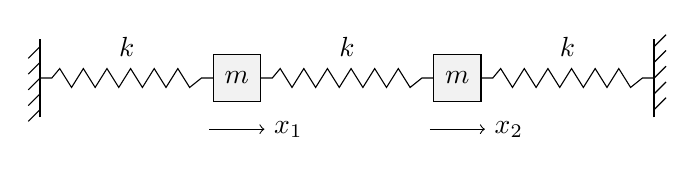
\begin{tikzpicture}[scale=1]
\foreach \s in {0,2.8,5.6}{
 \begin{scope}[shift={(\s,0)}]
 \draw (0,0)--(0.15,0)--(0.25,0.12)--(0.4,-0.12)--(0.55,0.12)
 --(0.7,-0.12)--(0.85,0.12)--(1,-0.12)--(1.15,0.12)
 --(1.3,-0.12)--(1.45,0.12)--(1.6,-0.12)--(1.75,0.12)
 --(1.9,-0.12)--(2.05,0)--(2.2,0);
 \node at (1.1,0.4) {$k$};
 \end{scope}
}
\draw[thick] (0,-0.5)--(0,0.5) (7.8,-0.5)--(7.8,0.5);
\foreach \y in {-0.4,-0.2,0,0.2,0.4}{
 \draw (0,\y)--(-0.15,{\y-0.15});
 \draw (7.8,\y)--(7.95,{\y+0.15});
}
\draw[fill=gray!10] (2.2,-0.3) rectangle (2.8,0.3);
\draw[fill=gray!10] (5,-0.3) rectangle (5.6,0.3);
\node at (2.5,0) {$m$};\node at (5.3,0) {$m$};
\draw[->] (2.15,-0.65)--(2.85,-0.65) node[right] {$x_1$};
\draw[->] (4.95,-0.65)--(5.65,-0.65) node[right] {$x_2$};
\end{tikzpicture}
\par\small Fig.~6.5 (schematic): equal masses and three equal spring constants.
\end{center}
\begin{enumerate}
\item[(a)] Set up the Newtonian acceleration equation for each mass.
\item[(b)] Solve the secular equation for the \erratum{eigenvalues}.
\item[(c)] Determine the eigenvectors and thus the normal modes of motion.
\end{enumerate}
\solution
The source figure has three springs with the same constant $k$ and
two masses of the same mass $m$. Take $m,k>0$ and measure both
displacements to the right from equilibrium.

(a) The left outer spring exerts $-kx_1$ on mass 1. The middle spring's
extension is $x_2-x_1$, so its forces are $+k(x_2-x_1)$ on mass 1 and
$-k(x_2-x_1)$ on mass 2. The right outer spring exerts $-kx_2$ on
mass 2. Newton's equations are therefore
\[
\boxed{m\ddot x_1=-2kx_1+kx_2,\qquad
       m\ddot x_2=kx_1-2kx_2.}
\]
In matrix notation,
\[
m\ddot{\boldsymbol x}+k
\begin{pmatrix}2&-1\\-1&2\end{pmatrix}\boldsymbol x=0.
\]
(b) Seek a normal mode
$\boldsymbol x(t)=\boldsymbol X e^{i\omega t}$ and use
$\ddot{\boldsymbol x}=-\omega^2\boldsymbol x$. Then
\[
\begin{pmatrix}2&-1\\-1&2\end{pmatrix}\boldsymbol X
=\lambda\boldsymbol X,
\qquad\lambda=\frac{m\omega^2}{k}.
\]
The secular equation is
\[
0=\begin{vmatrix}2-\lambda&-1\\-1&2-\lambda\end{vmatrix}
=(2-\lambda)^2-1
=\lambda^2-4\lambda+3=(\lambda-1)(\lambda-3).
\]
Thus
\[
\boxed{\omega_+=\sqrt{k/m},\qquad\omega_-=\sqrt{3k/m}.}
\]
\erratum{Part (b) asks for eigenvectors in the source; the secular
equation determines the eigenvalues. The eigenvectors are then found
in part (c), as follows.}

(c) For $\lambda=1$, the first row is $X_1-X_2=0$; choose the
unit vector $u_+=(1,1)^{\mathsf T}/\sqrt2$. The masses move in phase
with equal displacement, so the middle spring has no changing extension.
For $\lambda=3$, the first row is $-X_1-X_2=0$; choose
$u_-=(1,-1)^{\mathsf T}/\sqrt2$. The masses move with equal amplitudes
and opposite signs, stretching and compressing the middle spring.
These vectors have norm one and inner product zero.

The corresponding normal coordinates are
\[
Q_+=\frac{x_1+x_2}{\sqrt2},\qquad Q_-=\frac{x_1-x_2}{\sqrt2}.
\]
Adding and subtracting the Newton equations gives
\[
m\ddot Q_++kQ_+=0,\qquad m\ddot Q_-+3kQ_-=0.
\]
Therefore the general real motion can be written
\[
\boxed{\boldsymbol x(t)
=C_+u_+\cos(\omega_+t+\delta_+)
 +C_-u_-\cos(\omega_-t+\delta_-),}
\]
where the amplitudes and phases are fixed by the initial positions
and velocities.

\Needspace{5\baselineskip}
\par\bigskip
\noindent\textbf{6.5.20}\quad Given a normal matrix $\mathsf{A}$ with
eigenvalues $\lambda_{j}$, show that $\mathsf{A}^{\dagger}$ has eigenvalues
$\lambda_{j}^{*}$, its real part $(\mathsf{A}+\mathsf{A}^{\dagger})/2$ has
eigenvalues $\Re(\lambda_{j})$, and its imaginary part
$(\mathsf{A}-\mathsf{A}^{\dagger})/2i$ has eigenvalues $\Im(\lambda_{j})$.
\solution
First show that a right eigenvector of a normal matrix is also an
eigenvector of its adjoint with the conjugate eigenvalue. If
$Ax_j=\lambda_jx_j$, put $B=A-\lambda_jI$. It is normal because
\[
BB^\dagger-B^\dagger B=AA^\dagger-A^\dagger A=0.
\]
Using $Bx_j=0$, compute
\[
\|B^\dagger x_j\|^2
=x_j^\dagger BB^\dagger x_j
=x_j^\dagger B^\dagger Bx_j
=\|Bx_j\|^2=0.
\]
A vector with zero norm is zero, so
$B^\dagger x_j=0$, or $\boxed{A^\dagger x_j=\lambda_j^*x_j}$.
Now add and subtract the two eigenvalue equations:
\[
\frac{A+A^\dagger}{2}x_j
=\frac{\lambda_j+\lambda_j^*}{2}x_j
=\boxed{\Re(\lambda_j)x_j},
\]
\[
\frac{A-A^\dagger}{2i}x_j
=\frac{\lambda_j-\lambda_j^*}{2i}x_j
=\boxed{\Im(\lambda_j)x_j}.
\]
Thus the adjoint and both Hermitian parts share the original
orthonormal eigenbasis; the indicated eigenvalues follow on each basis
vector, including degenerate eigenspaces.

\Needspace{5\baselineskip}
\par\bigskip
\noindent\textbf{6.5.21}\quad Consider a rotation given by Euler angles
$\alpha=\pi/4$, $\beta=\pi/2$, $\gamma=5\pi/4$.
\begin{enumerate}
\item[(a)] Using the formula of Eq.~(3.37), construct the matrix $\mathsf{U}$
  representing this rotation.
\item[(b)] Find the eigenvalues and eigenvectors of $\mathsf{U}$, and from
  them describe this rotation by specifying a single rotation axis and an
  angle of rotation about that axis.
\end{enumerate}
\emph{Note.}~This technique provides a representation of rotations alternative
to the Euler angles.
\solution
(a) Equation (3.37), verified against textbook p.~141, uses
$U=S_3(\gamma)S_2(\beta)S_1(\alpha)$, where the rotations act on
coordinates. Set $c=1/\sqrt2$. The specified angles give
\[
\cos\alpha=\sin\alpha=c,\quad
\cos\beta=0,\quad\sin\beta=1,\quad
\cos\gamma=\sin\gamma=-c.
\]
The three matrices and their first product are
\[
S_1=\begin{pmatrix}c&c&0\\-c&c&0\\0&0&1\end{pmatrix},\quad
S_2=\begin{pmatrix}0&0&-1\\0&1&0\\1&0&0\end{pmatrix},\quad
S_3=\begin{pmatrix}-c&-c&0\\c&-c&0\\0&0&1\end{pmatrix},
\]
\[
S_2S_1=\begin{pmatrix}0&0&-1\\-c&c&0\\c&c&0\end{pmatrix}.
\]
Multiplying by $S_3$ on the left gives
\[
\boxed{U=\begin{pmatrix}
1/2&-1/2&1/\sqrt2\\
1/2&-1/2&-1/\sqrt2\\
1/\sqrt2&1/\sqrt2&0
\end{pmatrix}.}
\]
Its columns have norm one and pairwise scalar products zero; its
determinant is $1$, as also follows from the three proper-rotation
factors.

(b) To display the characteristic calculation without fractions,
expand the determinant of $2(U-\lambda I)$:
\begin{align*}
8\det(U-\lambda I)
&=\begin{vmatrix}
1-2\lambda&-1&\sqrt2\\1&-1-2\lambda&-\sqrt2\\
\sqrt2&\sqrt2&-2\lambda
\end{vmatrix}\\
&=(1-2\lambda)(4\lambda^2+2\lambda+2)
  +(2-2\lambda)+4(1+\lambda)\\
&=8(1-\lambda^3).
\end{align*}
Thus
\[
\lambda^3=1,\qquad
\boxed{\lambda_0=1,\quad
\lambda_\pm=\frac{-1\pm i\sqrt3}{2}=e^{\pm2\pi i/3}.}
\]
For an eigenvector $(x,y,z)^{\mathsf T}$, adding the first two rows of
the eigenvalue equation and retaining the third gives
\[
(1-\lambda)x-(1+\lambda)y=0,\qquad
x+y=\sqrt2\lambda z.
\]
At $\lambda=1$ the first equation gives $y=0$ and the second gives
$x=\sqrt2 z$. The remaining row also holds. Normalizing yields the
fixed-axis vector
\[
\boxed{n=\frac{(\sqrt2,0,1)^{\mathsf T}}{\sqrt3}.}
\]
For $\lambda=\lambda_\pm$, substitute
$y=\sqrt2\lambda z-x$ into the first equation:
\[
2x-\sqrt2\lambda(1+\lambda)z=0.
\]
Since $\lambda^2+\lambda+1=0$, this gives $x=-z/\sqrt2$ and then
\[
y=\frac{1+2\lambda}{\sqrt2}z
=\pm i\sqrt{\frac32}\,z.
\]
For $z=1$ the squared Hermitian norm is $1/2+3/2+1=3$, so
\[
\boxed{u_\pm=
\begin{pmatrix}-1/\sqrt6\\ \pm i/\sqrt2\\1/\sqrt3\end{pmatrix}.}
\]
Substitution into the unused row gives $Uu_\pm=\lambda_\pm u_\pm$.
Also $n^\dagger u_\pm=-1/3+1/3=0$ and
$u_+^\dagger u_-=1/6-1/2+1/3=0$, so these three vectors are
orthonormal.

The rotation axis is the line through the origin parallel to
$(\sqrt2,0,1)$, and its unsigned angle is $2\pi/3=120^\circ$.
The sign can be fixed, rather than inferred only from a conjugate pair
of eigenvalues. Define $[n]_\times v=n\times v$. Direct subtraction gives
\[
U-U^{\mathsf T}
=\begin{pmatrix}0&-1&0\\1&0&-\sqrt2\\0&\sqrt2&0\end{pmatrix}
=\sqrt3\,[n]_\times.
\]
For an active right-handed rotation, $R-R^{\mathsf T}
=2\sin\varphi[n]_\times$, while
$\operatorname{tr}U=0=1+2\cos\varphi$. Thus active application of $U$
to a column vector is a rotation by $+120^\circ$ about $n$.
\erratum{Equation (3.37) is a passive coordinate transformation.
The corresponding rotation of the coordinate axes is therefore
$-120^\circ$ about $n$, equivalently $+120^\circ$ about $-n$.
The directed angle must be paired with the chosen direction of the axis.}
